\documentclass[12pt]{article}

\usepackage[french]{babel} % Document en français
\usepackage[T1]{fontenc} % Suppression d'un warning
\usepackage[utf8]{inputenc} % Document UTF8
\usepackage{graphicx} % Insertion d'images
\usepackage[left=2.2cm, right=2.2cm, top=2.5cm, bottom=2.5cm]{geometry} % Mise en page
\usepackage{multicol} % Texte en multicolonnes avec multicols
\usepackage{placeins}
\usepackage{titling}
\usepackage{hyperref}

\graphicspath{{res/}}

\newcommand{\HRule}{\rule{\linewidth}{0.5mm}}

\begin{document}

\begin{titlepage}
\begin{center}

% Upper part of the page. The '~' is needed because \\
% only works if a paragraph has started.

\includegraphics[width=0.15\textwidth]{./logo_ucl.png}~\\[1cm]

\textsc{\LARGE Université catholique de Louvain}\\[1.5cm]

\textsc{\Large Notes de cours}\\[0.5cm]

% Title
\HRule \\[0.4cm]
{ \huge \bfseries LECGE1321 - Management humain \\[0.4cm] }

\HRule \\[1.5cm]

% Author and supervisor
\noindent
\begin{minipage}[t]{0.4\textwidth}
\begin{flushleft} \large
\emph{Auteurs :}\\
Florian \textsc{Thuin} \\
Eddy \textsc{Ndizera}
\end{flushleft}
\end{minipage}%
\begin{minipage}[t]{0.4\textwidth}
\begin{flushright} \large
\emph{Professeur :} \\
Nathalie \textsc{Delobbe}
\end{flushright}
\end{minipage}

\vfill

% Bottom of the page
{\large \today}

\end{center}
\end{titlepage}

%\maketitle
\tableofcontents

\newpage

\section{Introduction}
  \subsection{Le champ du management humain}
  \subsection{Un outil d'analyse : les niveaux d'Ardoino}
  Les niveaux d'intelligibilité d'Ardoino (fig.~\ref{niveau_ardoino}) sont un modèle d'analyse d'une réalité sociale. Celui-ci permet de mettre en défaut la pensée simpliste qui consiste à attribuer une erreur à un facteur individuel (\og{} erreur fondamentale d'attribution\fg{}). La théorie fondamentale de l'attribution consiste d'une part à attribuer sa propre réussite à soi-même et ses échecs à un contexte et d'autre part à attribuer la réussite des autres à un contexte et leurs échecs à eux-mêmes.
  
  Il y a 5 niveaux :
  
  \begin{enumerate}
   \item Le niveau individuel
   \item Le niveau relationnel et groupal
   \item Le niveau organisationnel
   \item Le niveau institutionnel
   \item Le niveau d'historicité
  \end{enumerate}
  
  \begin{figure}[h]
  	\begin{center}
  	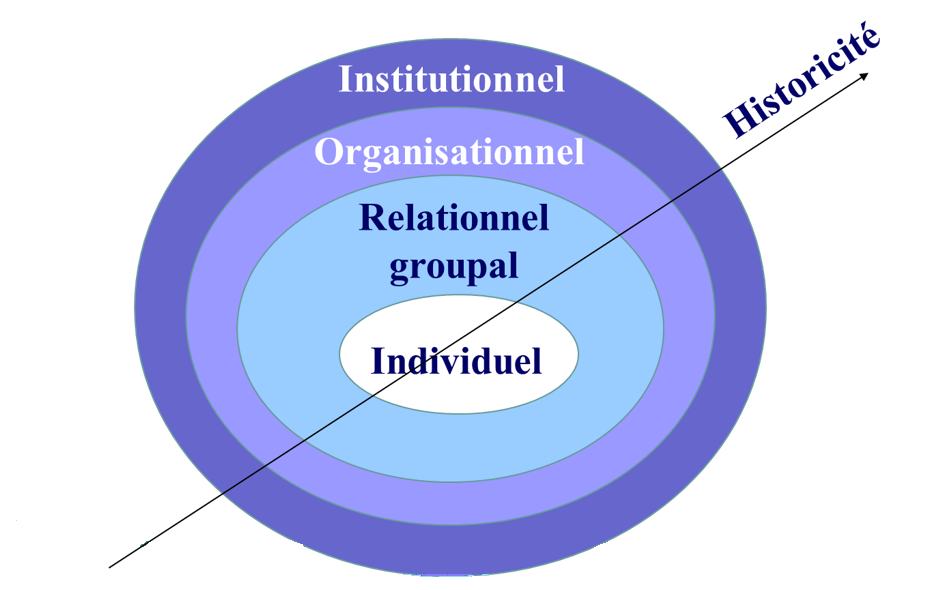
\includegraphics[scale=0.5]{niveau_ardoino}
  	\caption{Niveaux d'intelligibilité d'Ardoino}
  	\label{niveau_ardoino}
   	\end{center}
  \end{figure}
  
  \begin{description}
   \item[Niveau individuel] : les facteurs individuels d'ordre psychologiques (attitude, caractère, personnalité, motivations,...)
   \item[Niveau relationnel et groupal] : les relations interpersonnelles et affectives (la communication). Ce niveau étudie les phénomènes de groupe : cohésion, appartenance, esprit de groupe, amitié, complicité, conflits interpersonnels.
   \item[Niveau organisationnel] : les modalités d'organisation de l'action collective. Ce niveau étudie les problèmes d'efficacité : les règles, lee rôles, les status, les modes de division et de coordination du travail, la structure du pouvoir,... 
   \item[Niveau institutionnel] : les valeurs, les normes, la culture. Ce niveau étudie les institutions publiques, les cadres politique, juridique, social et économique ainsi que les règles formelles (lois) et informelles (culture, traditions) qui régissent l'ensemble de la société.
   \item[Niveau d'historicité] : analyse des autres dimensions à travers l'histoire. Ce niveau étudie les transformations de la société, les mouvements sociaux, les tendances économiques, les rapports de force entre les classes sociales,...
  \end{description}
  \subsection{Cas type : France Telecom}
  
  Si on applique le modèle d'Ardoino sur le phénomène de vague de suicides qu'à connu France Télécom\footnote{\url{https://www.youtube.com/watch?v=YBXp45yYIA8}}, on obtient ceci:
  \begin{enumerate}
  \item \textbf{Individuel}:    \begin{itemize}
  								\item préférences
  								\item vie personnelle
  								\item PDG remis en question
  								\end{itemize}
  \item \textbf{Relationnel et groupal}:    \begin{itemize}
  											\item effet de mode pour le suicide
  											\item abus de pouvoir de la hiérarchie
  											\item isolement au travail, liens sociaux rompus
  											\item communication très autoritaire avec peu de dialogue (leadership autoritaire)
  											\end{itemize}
  \item \textbf{Organisationnel}:   \begin{itemize}
  									\item plan de mobilité du personnel
  									\item changement de culture, on passe d'une entreprise public à une entreprise privée
  									\item hiérarchie forte
  									\item le passage de public à privé pousse à une réorganisation des sources financières (70\% masse salariale)
  									\end{itemize}
  \item \textbf{Institutionnel}:  	\begin{itemize}
  									\item gestion du personnel sortant du cadre juridique français (on devient plus nord-américain), tradition d'écoute du salarié
  									\item marché du travail rigide
  									\item changement de statut des travailleurs (avant, fonctionnaires pas de licenciement)
  									\end{itemize}
\end{enumerate}   
  \subsection{Management humain : de quoi parle-t-on ?}
    \subsubsection{People management}
      Le people management correspond à l'encadrement des employés et au leadership par différents moyens :
      
      \begin{itemize}
       \item Organisation et coordination du travail
       \item Supervision et développement des individus
       \item Animation et conduite des équipes
      \end{itemize}
    
    \subsubsection{Gestion des ressources humaines}
      
      La gestion des ressources humaines est plus formalisée et a pour thèmes :
      
      \begin{itemize}
       \item Le recrutement et la sélection
       \item L'allocation et la planification des ressources humaines
       \item La classification des emplois et les rémunérations
       \item Le développement des employés et les formations
       \item L'évaluation des performances
       \item Le dialogue social et la communication
      \end{itemize}
      
  \subsection{Le modèle de Kolb}
  
  L'activité d'un manager dans les RH peut être représentée par le modèle de Kolb (fig.~\ref{modele_kolb}).
  
  \begin{figure}[h]
  	\begin{center}
  	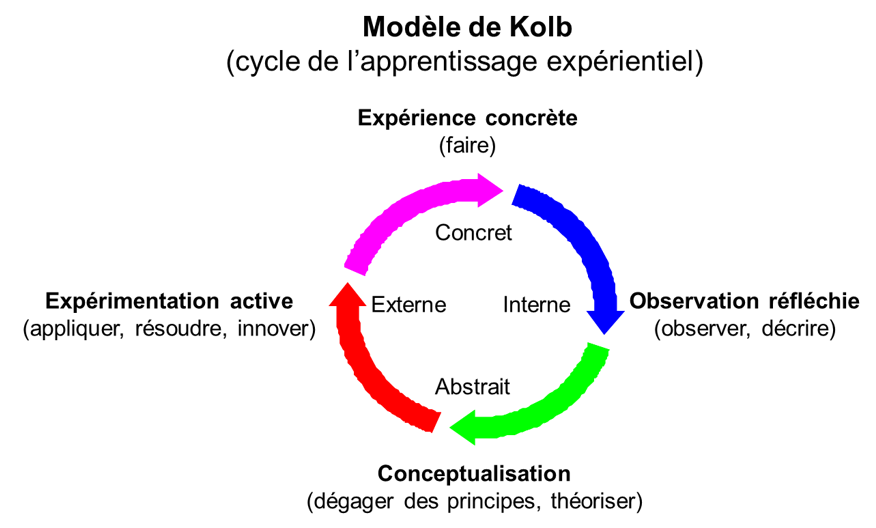
\includegraphics[scale=0.6]{modele_kolb.png}
  	\caption{Modèle de Kolb}
  	\label{modele_kolb}
  	\end{center}
  \end{figure}
  
  \subsection{Structure générale du cours}
    Le cours se partage en deux axes.
    
    \paragraph{Axe historique}
      \begin{enumerate}
       \item L'administration du personnel
       \item L'école des relations humaines
       \item Le courant socio-technique
       \item La gestion stratégique des ressources humaines
      \end{enumerate}
    
    \paragraph{Axe thématique}
      \begin{enumerate}
       \item L'engagement et la motivation au travail
       \item Le pouvoir, l'autorité et le leadership
       \item La dynamique et les facteurs d'efficacité dans les groupes et équipes
       \item Les valeurs et la culture dans les organisations
      \end{enumerate}

\section{Panorama historique et rôles de la fonction RH}
	\subsection{Les étapes historiques}
	  \begin{itemize}
	   \item Contextes socio-économiques distincts
	   \item Modèles dominants d'organisation du travail et de pensée stratégique
	   \item Conceptions sous-jacentes de l'être humain
	   \item Rôles distincts pour la fonction RH
	   \item Champs de préoccupations et de pratiques RH
	  \end{itemize}
	  
	  \subsection{Les 4 rôles RH (D. Ulrich, 1993)}
	  
	  \begin{enumerate}
	   \item Expert administratif
	   \item Champion des employés
	   \item Agent de changement
	   \item Partenaire stratégique
	  \end{enumerate}

	  \begin{figure}[h]
	  	\begin{center}
	  	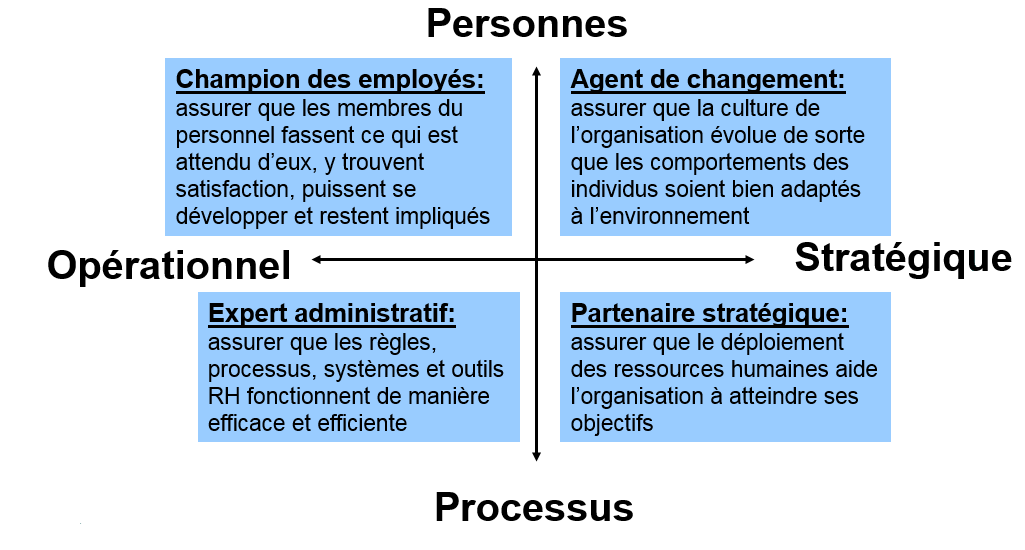
\includegraphics[scale=0.5]{modele_ulrich.png}
	  	\caption{Les 4 rôles RH (D.Ulrich, 1993).}
	  	\label{modele_ulrich}
	  	\end{center}
	  \end{figure}
	  
	  Comme on peut le voir sur la figure ~\ref{modele_ulrich}, l'axe \textbf{opérationnel} tient compte plus des objectifs internes à l'entreprise tandis que l'axe \textbf{stratégique} prend en compte plus la survie à l'environnement auquel évolue l'entreprise. De plus, une entreprise peut être centré davantage sur les \textbf{personnes} ou bien sur l'efficience (\textbf{processus}), intérêts économiques.\newline
	  
	  \begin{description}
	   \item[Expert administratif] : rôle centré sur la surveillance des contrats de travail et des règlements (processus et résultats)
	   \item[Champion des employés] : rôle centré sur la motivation des employés (la personne et son développement).
	   \item[Agent de changement] : rôle centré sur l'adaptation et l'évolution de l'organisation et des hommes (stratégies, approche socio-technique)
	   \item[Partenaire stratégique] : rôle centré sur la plus-value et les succès stratégiques de l'organisation (processus et résultats)
	  \end{description}
	  
	\subsection{L'administration du personnel}
	Les fondements de la fonction RH
	  \subsubsection{Le contexte socio-économique}
	  On est en pleine révolution industrielle (18-19ème siècle) dont les principales caractéristiques sont :
	  
	  \begin{itemize}
	   \item Progrès technologique : le machinisme, l'industrialisatio massive de la production ;
	   \item Disparition des corporations de métiers ;
	   \item Patron arbitraire, paternaliste ;
	   \item Avènement de l'entreprise capitaliste ;
	   \item Construction d'un marché de libre échange ;
	   \item Naissance des valeurs démocratiques républicaines ;
	   \item Dualisation de la société : bourgeoisie industrielle VS prolétariat
	   \item Perte d'autonomie et déqualification progressive des travailleurs
	   \item Conditions de travail misérables et précarisation économique de la classe ouvrière
	  \end{itemize}
	  
	  Cette période correspond également la naissance du mouvement ouvrier et du syndicalisme : nouvelle législation et apparition de la concertation sociale.

	  \subsubsection{Les modèles d'organisation du travail}
	  
	  \paragraph{L'organisation scientifique du travail (Taylorisme)}
	  \begin{description}
	   \item[Standardisation] : parcellisation et simplification des tâches (chronométrage des temps et mouvements).
	   \item[Distinction conception-exécution] : pour augmenter le rendement et la qualité de vie des ouvriers.
	  \end{description}
	  
	  \paragraph{Bureaucratie Wéberienne}
	  \begin{description}
	   \item[Formalisation et impersonnalité] : la règle remplace la tradition et l'arbitraire.
	   \item[Centralisation et hiérarchisation] : structure hiérarchique conforme au principe d'unité de commandement (= un agent ne doit recevoir des ordres que d'un seul chef) \newline
	  \end{description}
	  
		La bureaucratie Wéberienne veut donc que les règles soient les mêmes pour tout le monde. De plus chaque membre devrait relever d'un supérieur hiérarchique.
	  
	  \subsubsection{Les options stratégiques}
	  \begin{description}
	   \item[Fordisme] : gains en productivité et croissance assurés par une production et une consommation de masse.
	   \item[Planification rationnelle] : (one best way = la seule bonne façon de gérer) dans un environnement stable et peu compétitif. 
	  \end{description}

	  \subsubsection{La conception de l'homme}
	  
	  L'homme était vu comme une main d'oeuvre vite opérationnelle et substituable. C'est l'époque de la dominance \textit{behavioriste} en psychologie industrielle.
	  
	  Le behaviorisme est la concentration sur le comportement observable déterminé par l'environnement et l'histoire des interactions de l'individu avec son milieu, sans faire appel à des mécanismes internes.
	  
	  \emph{Postulat de l'homme économique} : un être paresseux attiré par les stimulations monétaires, irrationnel dont il faut organiser, planifier, contrôler le travail.
	  
	  \emph{Forme d'intégration} : engagement calculé, fondé sur des incitants extrinsèques (comme le fait de vouloir éviter le chômage).
	  
	  \subsubsection{Conception de la fonction RH}
	  
	  C'est \emph{l'expert administratif} (selon D. Ulrich) : \og{} bureau du personnel \fg{}
	  
	  \begin{itemize}
	   \item Administration des contrats de travail ;
	   \item Conception des systèmes de contrôle formel (règles, blâmes, ...) ;
	   \item Elaboration des systèmes de rémunérations/incitations et gestion de paie (payroll) ;
	   \item Prévention et gestion des conflits sociaux (concertation sociale). 
	  \end{itemize}
	  
	  Le profil du DRH est un ingénieur (optimisation des processus) et un juriste (contrats et conflits).
	  
	  \subsubsection{Pratiques héritées de la RH}
	  
	  \begin{itemize}
	   \item Analyse du travail et description de poste ; \newline
	   ex: Le chronométrage du temps pour les tâches issus de l'organisation scientifique du travail (Taylor).
	   \item Développement de la réglementation sociale (règlement de travail, droit social) ;
	   \item Développement de la concertation sociale en réponse au mouvement ouvrier et au syndicalisme
	   \item Classification des emplois et barèmes salariaux ;
	   \item Sécurité physique et hygiène
	  \end{itemize}

	\subsection{L'école des relations humaines}
	La gestion de l'homme au travail.
	  \subsubsection{Contexte socio-économique}
	  
	  Le \textbf{contexte socio-économique est stable}, il n'y a pas de remise en cause du modèle productif.
	  
	  La \textbf{croissance économique} permet des stratégies de croissance par intégration des activités (en amont et en aval), la diversification mais entraîne des difficultés croissantes de coordination et d'intégration interne.
	  
	  Une \textbf{nouvelle classe} sociale apparaît : les cadres intermédiaires qui ont pour mission d'assurer la coordination et l'intégration dans des groupes de travail.
	  
	  On s'oriente vers des \emph{structures mécanistes divisionalisées}.
	  
	  \subsubsection{Expérience de la Western Electric (1927)}
	  
	  Elton Mayo enquête sur le rendement dans une entreprise.
	  
	  \begin{table}[!ht]
	        \begin{tabular}{p{4.7cm}|p{7.3cm}|p{3.5cm}}
		Phase & Action & Rendement \\
		\hline \hline
		1ère phase (15 semaines) & Salaire d'équipe aux pièces & 2500 relais/semaine \\ \hline
		2ème phase (24 semaines) & Expérimentation d'un système de pauses intercalaires & 2600 relais/semaine \\ \hline
		3ème phase (32 semaines) & Réduction de la journée puis de la semaine de travail (5 jours) & 2800 relais/semaine \\ \hline
		4ème phase (12 semaines) & Suppression des pauses et de la collation, rétablissement de la semaine de 48 heures sur 5 jours & 2900 relais/semaine \\ \hline
		5ème phase (39 semaines) & Rétablissement des pauses avec une boisson & 3000 relais/semaine \\ \hline
	    \end{tabular}
	    \caption{Résultats de l'expérience d'Elton Mayo}
	  \end{table}
	  
	  Quels sont les facteurs explicatifs ?
	  
	  \begin{description}
	   \item[Les incitants autres que pécuniaires] : reconnaissance, valorisation sociale
	   \item[Leadership] : un style de commandement plus libéral et un leadership plus informels
	   \item[Dynamique informelle des groupes] : cohésion sociale, objectifs partagés, solidarité et appartenance.
	  \end{description}
	  
	  \subsubsection{Conception de l'homme}
	  
	  \begin{itemize}
	   \item Behavioriste
	   \item Le personnel est intrinsèquement motivé et loyal
	   \item Courant humaniste dominant (Carl Rogers)
	   \item L'homme est en quête de réalisation
	    \subitem doté de besoins à assouvir et capable d'auto-régulation
	    \subitem Dimensions socio-affectives de l'être humain
	   \item Engagement affectif de l'homme dans l'entreprise
	  \end{itemize}

	  
	  \paragraph{Behaviorisme} L'être humain ne peut être connu que de l'extérieur. L'intérieur est une \og{} boîte noire\fg{}. Pour découvrir ce qu'il y a dans cette boîte noire, on utilise des stimuli et on regarde le changement de rendement. Les gens se sont sentis pris en considération par l'étude, écoutés, entendus (\textbf{incitants non pécuniaires}). Le leader dans le groupe de personnes analysées était la doyenne de l'entreprise, c'est un \textbf{leadership informel}.
	  
	  \paragraph{Forme d'intégration} L'homme est dans un engagement affectif dans l'entreprise, il peut subir des stimulations fondées sur la motivation, la réalisation de soi, la recherche de changement, la reconnaissance et l'appartenance sociale.
	  
	  Globalement, on peut dire que l'homme n'est plus uniquement motivé par des besoins économiques mais que des besoins socio-affectifs affectent également sa productivité.
	  
	%TODO illustration théorie X et Y 	  
	  \subsubsection{Conception de la fonction RH}
	  
	  Le DRH est \og{} champion des employés\fg{} (selon D. Ulrich) : directeur des relations humaines.
	  
	  Sa fonction sera de gérer les gens à la fois par les intérêts économiques et la prise en considération d'eux en tant qu'humain. Il doit concilier les intérêts économiques et les aspirations individuelles :
	  
	  \begin{itemize}
	   \item Répondre aux besoins et préoccupations des employés ;
	   \item Assurer leur motivation et leur contribution aux objectifs de l'entreprise (nouveau par rapport au Taylorisme)
	   \item Le travailleur satisfait est plus productif
	  \end{itemize}
	  
	  Le profil du DRH s'oriente maintenant davantange vers le \emph{psychologue}.
	  
	  \subsubsection{Pratiques héritées}
	  
	  Cette période correspond au développement des fonctions-clés de la GRH :
	  
	  \begin{itemize}
	   \item \textbf{Sélection} sur base de dimensions \textbf{psychologiques} (motivations, aspirations,...).
	   \item \textbf{Formation} aux relations humaines (leadership,...). Dans l'Organisation Scientifique du Travail, la formation est très rapide et minimum. Ici les pratiques de formation sont plus larges et basées sur des dispositions plus psychologiques.
	   \item \textbf{Evaluation} du personnel et MBO : management by objective = différence entre tâche (chose à réaliser) et objectif (résultat visé). On vérifie maintenant si le personnel effectue ce qui lui est demandé et non plus le temps.
	   \item Gestion des \textbf{carrières} : importance des cadres dans les grosses entreprises (proposer des perspectives de carrière).
	   \item \textbf{Communication} interne via gazette pour informer et sensibiliser le travailleur.
	   \item Enquête de \textbf{climat social} et développement de la culture d'entreprise.
	  \end{itemize}
	  
	\subsection{L'approche socio-technique}
	Au coeur du développement social de l'organisation.
	
	\subsubsection{Contexte socio-économique}
	
	On est dans un contexte d'après-guerre :
	
	\begin{itemize}
	 \item Accélération des changements technologiques (début de l'informatisation et de la robotisation)
	 \item Saturation de la production de masse pour certains marchés et accent sur de nouveaux critères de compétitivité : qualité totale, variété, délais,...
	 \item Révolution culturelle de Mai 68 et aspirations à une société plus démocratique
	\end{itemize}
	
	On passe à une approche socio-technique du changement (amélioration de la production), l'organisation mécaniste devient flexible, développement d'un management de qualité globale, d'approches participatives et de démocratie organisationnelle.
	
	L'histoire vit son premier choc pétrolier (1973) lors duquel les prix de l'essence quadruple. On envisage que les ressources ne sont pas inépuisables et qu'un modèle de croissance illimité ne fonctionne pas.
	
	\subsubsection{Modèle de l'organisation du travail}
	De l'entreprise mécanique à l'entreprise organique.
	
	La \textbf{division du travail} se fait sur deux niveaux :
	\begin{enumerate}
	 \item Verticalement (par niveaux hiérarchiques) : fortement mécanique et faiblement organique
	 \item Horizontalement (par départements) : division mécanique et intégration organique
	\end{enumerate}
	
	La \textbf{coordination du travail} varie selon la division réalisée mais tend à :
	\begin{enumerate}
	 \item la stabilisation des procédures
	 \item la stabilisation des résultats et des qualifications
	 \item l'autorégulation, l'ajustement mutuel
	\end{enumerate}
	
	La \textbf{départementalisation} se fait
	\begin{enumerate}
	 \item par fonction (\emph{mécanique})
	 \item par marché ou produit (\emph{organique})
	\end{enumerate}
	
	On développe la \textbf{liaison entre unité} par
	\begin{enumerate}
	 \item la planification et le contrôle
	 \item la création de \og{} task force\fg{} : des groupes crées pour un projet précis
	\end{enumerate}
	
	Le \textbf{degré de centralisation} est élévé :
	\begin{enumerate}
	 \item contrôle par les ingénieurs
	 \item décisions stratégiques
	\end{enumerate}
	mais est faible pour les décisions opérationnelles (besoin de flexibilité)
	
	Les \textbf{acteurs influents} (selon Minzberg) sont
	\begin{enumerate}
	 \item Les analyses et les experts de la technostructure (ingénieur,...)
	 \item Le centre opérationnel plus proche du client (organique)
	\end{enumerate}
	
	Les \textbf{buts prédominants} sont :
	\begin{enumerate}
	 \item des buts de système : maintien de la compétitivité et du rendement
	 \item des buts de mission : adaption de l'entreprise à son environnement
	\end{enumerate}
	
	L'\textbf{environnement} est différent :
	\begin{enumerate}
	 \item Soit il est stable, homogène, simple et peu hostile : on fait une planification à long terme
	 \item Soit il est instable, hétérogène et hostile : on doit s'adapter à la concurrence
	\end{enumerate}

	\subsubsection*{Expérience de Trist \& Bamforth}
	
	L'étude de E.Trist \& K.Bamforth opère autour d'une mine de charbons dont on automatise le transport (installation de wagonnets). Ce qu'ils constatent, c'est que ceci à pour effet de décroître la production. On est moins productif alors que tout mène à penser que le fait d'installer des wagonnets pour transporter le charbons devrait faciliter la tâche des travailleurs. \newline
	
	Selon Trist et Bamforth, cet effet néfaste a pour explications qu'on a touché, avec l'automatisation du transport, profondément au système social. En effet, dans ce milieu de mineurs très anxiogène, il y avait tout un imaginaire entre ces mineures. Il y avait un implicite collectif, un état d'esprit qui permettait à ces derniers de faire face à l'anxiété. Mais avec l'installation de wagonnets, les équipes se sont vu passer de 6 à 2. \newline
	
	Ce phénomène est aussi observable dans la Poste. En effet, il y a eu un grand débat avec l'installation d'un logiciel "\textit{géroute}" qui avait comme fonction de calculer les parcours pour les postiers. Ceci a eu pour effet de toucher aussi le système social des postiers. En effet, les postiers ne disposent plus des 2 heures de papotages qu'ils avaient avant quand ils triaient le courrier. Ceci est automatisé maintenant. Ils arrivent au boulot, ils ont déjà leurs lettres bien triés. Leurs parcours étant prédéfini désormais, il n'y a plus ces arrangements quand il s'agit de laisser Pierre faire la tournée de telle ville afin de pouvoir voir sa mère. \newline
	
	%Mieux expliquer cette phrase
	Ce système est toutefois dynamique. Il peut s'adapter.\newline
	
	La \textbf{méthodologie de recherche-action} est, dans le cas de la Poste, de soumettre aux postiers le problème (on doit être plus efficace) et les différentes solutions (géoroute). Ceci afin d'ouvrir une discussion avec les personnes concernées pour prendre mieux en compte les différents éléments à prendre au jeu. 
	
	
	\subsubsection{Conception de l'homme}
	L'homme est collaborateur et acteur au sens politique du terme. Le courant stratégique et politique est dominant en sociologie des organisations
	
	Le pouvoir n'est pas un attribut personnel, individuel, c'est le jeu d'une relation entre deux individus en interaction. C'est la capacité de faire quelque chose à l'autre, ce n'est pas quelque chose que seuls les dirigeants détiennent (Crozier \& Friedberg, 1977).
	
	\paragraph{Postulat de l'homme stratège} L'homme stratège a la rationalité limitée ($\neq$ irrationnel) et poursuit des intérêts particuliers. Il est un acteur et analyse une situation sociale (ou économique). Et, au contraire de la théorie économique (= examiner toutes les possibilités pour faire un choix), dès qu'on rencontre une \og{} solution\fg{} qui nous convient, on arrête l'analyse.
	
	Il est capable d'auto-détermination et est soucieux de l'influence politique.
	
	\paragraph{Forme d'intégration} L'organisation est considérée comme le lieu de nécessaire conciliation entre intérêts divergents.
	
	\subsubsection{Conception de la fonction RH}

	Le RH est vu comme un \og{} agent de changement\fg{} (selon D. Ulrich) avec le département du développement social. C’est un facilitateur interne, il accompagne les changements organisationnels, les réorganisations et l’introduction de nouvelles technologies.
	
	Le profil du DRH correspond à un consultant interne, un gestionnaire de projet.
	
	\subsubsection{Les pratiques héritées}
	
	Une nouvelle forme d’organisation du travail (NFOT) : les équipes semi-autonomes de production.
	
	De nouvelles démarches participatives d’amélioration et de changement :
	
	\begin{itemize}
		\item Cercles de qualité et qualité totale en réponse aux attentes individuelles des clients.
		\item Développement organisationnel : accompagnement d’équipes de travail afin de le définir.
		\item \og{}Business Process/Re-engineering\fg{} : repenser/réorganiser de façon radicale les étapes du processus de production des B/S. On suggère que cela est fait avec les acteurs concernés (démarche participative).
	\end{itemize}
	
	\subsection{La gestion stratégique des ressources humaines}
	Et l’homme devient une ressource stratégique...
		\subsubsection{Le contexte économique}
		\begin{enumerate}
		 \item Récession économique
		 \item Mondialisation
		 \item Déclin du secteur secondaire au profit du secteur tertiaire
		\end{enumerate}
		
		La \textbf{récession économique} touche les économies occidentales et provoque un divorce de l'économique et du social. Elle marque la fin de la sécurité de l'emploi, une crise du syndicalisme et un repli individualiste.
		
		La \textbf{mondialisation} rend non-compétitives les industries occidentales sans qualification requise et l'économie se transforme vers une économie \emph{de la connaissance et de l'innovation}.
		
		Le \textbf{déclin du secteur secondaire} à cause de la modification se fait au profit du développement du secteur tertiaire (les services) et du secteur quaternaire (services de proximité).
		
		\subsubsection{Modèle d’organisation et pensée stratégique}
		
		\begin{enumerate}
		 \item Théorie du capital humain
		 \item Recentralisation interne des entreprises
		 \item Flexibilité du marché du travail
		 \item Flexibilité des modes d'organisation du travail
		\end{enumerate}
		
		La \textbf{théorie du capital humain} désigne trois éléments qui déterminent l'aptitude d'un individu à travailler :
		
		\begin{itemize}
		 \item Les compétences ;
		 \item les expériences ;
		 \item et les savoirs
		\end{itemize}
		
		Tout comme pour les théories du capital financier et physique, le capital humain peut s'acquérir (éducation), se préserver et se développer (formation continue) et produire un bénéfice (travail).
		
		On assiste à une dualisation du personnel : ceux qui détiennent le \textbf{capital humain spécifique} (des compétences non-transférables) et ceux qui détiennent le \textbf{capital humain générique} (des compétences transférables).
		
		Les entreprises se \textbf{recentrent} sur les \og{} core competences \fg{}, autrement dit leurs activités centrales. Les autres parties sont externalisées, vendues, fusionnées avec d'autres entreprises,...
		
		On assiste à une \textbf{flexibilisation du travail} par la création de nouveaux types de contrats pour les employés.
		
		On assiste à une \textbf{flexibilisation des modes d'organisation du travail} avec l'apparition de l'adhocratie et des entreprises-réseaux.
		
		\subsubsection{Conception de l’homme au travail}
		
		L'homme devient un actif spécifique, une approche économique des RH se développent.
		
		C'est l'apparition du postulat de \og{} l'agent économique opportuniste \fg{} qui soutient que l'homme pense \og{} si on m'offre mieux ailleurs, je vais ailleurs \fg{}. Cela produit l'éclatement des sources d'attachement et la crise des identités au travail. C'est le début des carrières nomades : l'homme se déplace en fonction des opportunités et n'est plus lié à une organisation (il reste cependant lié à ses collègues et son métier).
		
		\subsubsection{Conception de la GRH}
		
		Le GRH devient \og{} partenaire stratégique \fg{} (selon D. Ulrich), il devient \emph{directeur des ressources humaines}. Les ressources humaines sont considérées comme une valeur ajoutée à la politique de l'entreprise, marquées par une individualisation et une segmentation du lien salarial et des pratiques RH.
		
		Le DRH devient un gestionnaire à part entière, il est membre du comité de direction qui doit optimiser la valeur des RH.
		
		\subsubsection{Pratiques en cours de développement}
		
		Cette partie historique étant encore en cours de développement, il est difficile de faire la part des choses puisqu'on est à la fois acteur et observateur. Cependant, on peut ressortir certaines pratiques :
		
		\begin{enumerate}
		 \item Gestion des compétences :
		    \subitem sélection ;
		    \subitem carrière ;
		    \subitem formation ;
		    \subitem évaluation
		 \item Individualisation des formes de rémunération
		 \item Diversification des statuts d'emploi :
		    \subitem intérim
		    \subitem sous-traitance
		 \item Tableaux de bords sociaux
		 \item Externalisation des opérations administratives
		 \item eRH : gestion électronique des RH
		\end{enumerate}

		
	\subsection{En bref\ldots}
	
	  % TODO : Ajouter les temps consacrés aux différents rôles
	  %TODO : expliquer figure
	  \begin{figure}[h]
	  	\begin{center}
	  	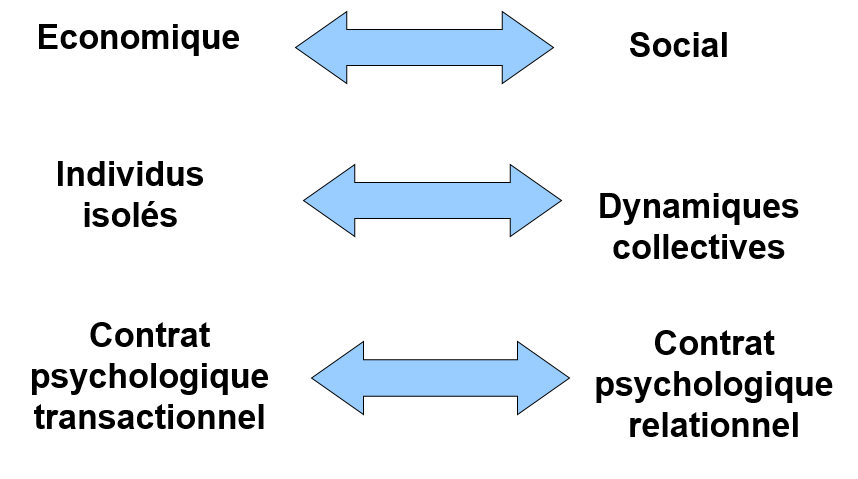
\includegraphics[scale=0.5]{tensions_fonction_RH.png}
	  	\caption{Tensions inhérentes à la fonction RH.}
	  	\end{center}
	  \end{figure}

\section{Culture organisationnelle}
	\subsection{Historique}
	\subsection{Le modèle de l'oignon d'Edgar Schein}
	
	Le modèle d'Edgar Schein est une conceptualisation de la notion de culture d'entreprise via une approche anthropologique.
	
	Pour Edgar Schein, la culture organisationnelle se définit comme \og{} un ensemble de prémisses et de croyances partagées que le groupe a appris au fur et à mesure qu'il a résolu ses problèmes d'adaptation externe et d'intégration interne, qui a fonctionné suffisamment bien pour qu'il soit considéré valide, et par conséquent est enseigné aux nouveaux membres comme la manière appropriée de percevoir, de penser et de ressentir par rapport à ces problèmes \fg{} \cite{schein2010}
	
	  \subsubsection{Un phénomène multi-niveaux}
	  
	  Edgar Schein divise la culture d'une entreprise en plusieurs niveaux :
	  
	  \begin{multicols}{2}
	  
	  Les \textbf{artéfacts} sont les aspects visibles de la culture : la manière de s'habiller, les logos, le jargon, l'humour,... Ils sont faciles à identifier par une démarche ethnographique mais il est difficile d'en tirer une signification sans analyser les autres niveaux de l'oignon.
	  
	  Les \textbf{valeurs} sont les stratégies, les objectifs et philosophies choisies de manière consciente et qui sont diffusées par la direction et le management de l'entreprise : compétitivité, solidarité, adaptation au changement, stabilité, etc.
	  
	  Les \textbf{normes de pensée et d'action} correspondent aux routines comportementales, habitudes, modèles d'action, rituels et schémas cognitifs d'inteprétation des évènements. Elles sont directement déterminées par les valeurs sous-jacentes.
	  	  
	  \begin{center}
	    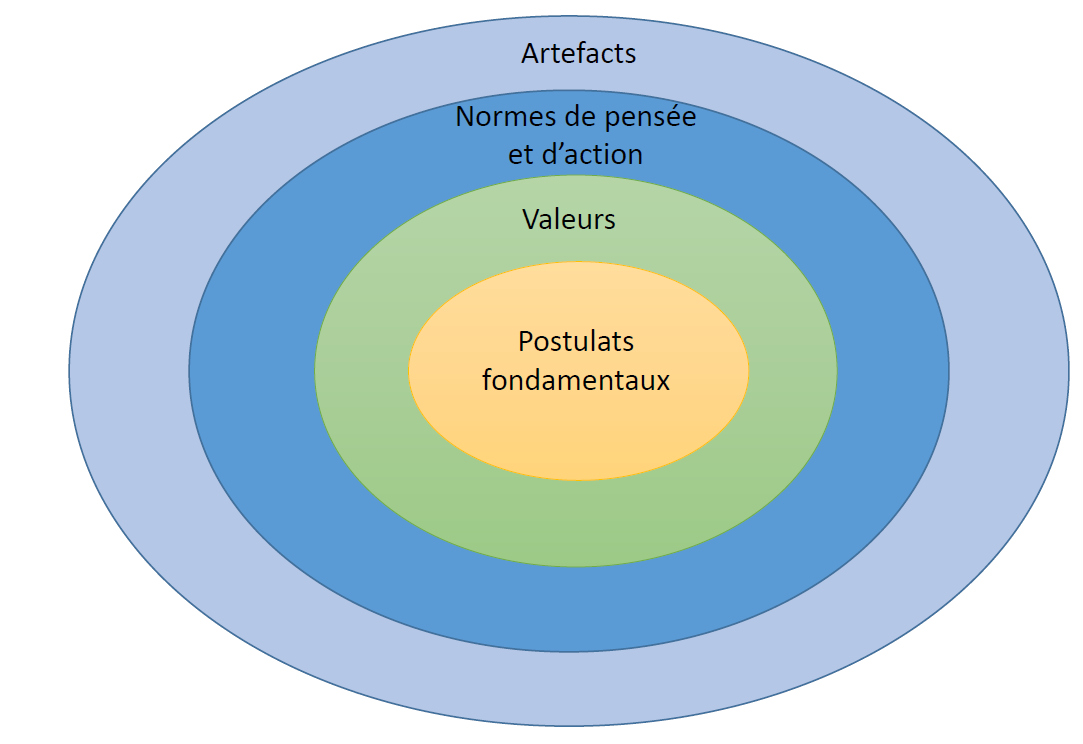
\includegraphics[width=\linewidth]{culture_orga_niveaux.png}
	  \end{center}
	  Les \textbf{postulats fondamentaux} ou prémisses sont les croyances qui sont l'essence de la culture. Ces prémisses sont difficiles à discerner car elles opèrent au niveau de l'inconscient. Elles portent sur des questions telles que la nature de l'homme, le rapport au temps, la notion de vérité, etc. Elles ne sont quasiment jamais remises en cause.
	  
	  Les artéfacts découlent des valeurs et les valeurs découlent des postulats fondamentaux.
	  
	  \end{multicols}
	  
      \subsection{Le modèle des valeurs concurrentes de Quinn}
	Ce modèle a été développé à l'origine pour décrire les valeurs sous-jacentes aux critères d'efficacité organisationnelle.
	
	Il caractérise les cultures organisationnelles selon 2 dimensions : le contrôle VS la flexibilité et les relations (interne) VS les résultats (externe).
	
	\subsubsection{Un phénomène multi-dimensionnel}
	
	  Quinn définit 4 grands types de cultures :
	  
	  La \textbf{culture de soutien} qui privilégie la coopération, la participation, l'attachement à l'entreprise, la communication interpersonnelle. C'est une culture de \og{} collaborateurs \fg{} qui peut se retrouver notamment dans les PME familiales.
	  
	  La \textbf{culture des règles} qui est très respectueuse des procédures, tout est écrit, tracé, standardisé. La communication est essentiellement descendante dans l'organigramme, c'est une culture \og{} d'organisateurs \fg{}. Cette culture peut se retrouver dans les administrations publiques.
	  
	  La \textbf{culture des buts} privilégie les objectifs de performance et la rationalisation des processus en vue des objectifs. C'est une culture de \og{} compétiteurs \fg{}. 
	  
	  La \textbf{culture de l'innovation} qui privilégie la créativité, l'ouverture au changement, l'expérimentation et l'adaptation permanente. La communication est aussi peu formalisée que possible pour casser la hiérarchie stricte, c'est une culture \og{} d'innovateurs \fg{}.
	  
	  Ce modèle peut se superposer à celui d'Ulrich pour tracer un historique des pratiques de ressources humaines.
	
	\subsection{La théorie des dimensions culturelles (1991)}
	
	Une organisation (de taille conséquente) n'est pas liée à une seule culture, il existe des sous-cultures. Il y a les sous-cultures par département, par métiers, par âge, par affinités,...
	
	  \subsubsection{Un phénomène hétérogène}
	  
	  Le modèle de Hofstede a pour but d'étudier les interactions entre les cultures en fonction de certaines dimensions en leur attribuant des scores de 1 à 120.
	  
	  Il met en avant 4 dimensions :
	  
	  \begin{enumerate}
	   \item Distance au pouvoir
	   \item Evitement de l'incertitude
	   \item Masculinité contre féminité
	   \item Individualisme contre collectivisme
	  \end{enumerate}
	  
	  La \textbf{distance au pouvoir} est un indice d'acceptation de pas avoir de pouvoir par les membres les plus éloignés de la direction dans l'organigramme.
	  Un indice faible signifie que les membres souhaitent une gestion démocratique et se considèrent à égalité avec les autres, un indice élevé indique que ceux qui ont le moins de pouvoir acceptent leur condition et sont forts soumis au pouvoir.
	  
	  L'\textbf{évitement de l'incertitude} correspond au degré de tolérance d'une société pour l'incertitude/l'ambiguité. Les sociétés avec un indice faible sont ouvertes aux changements, disposent de moins de règles et de lois et les directives y sont plus souples.
	  
	  La \textbf{masculinité contre la féminité} correspond au niveau d'importance accordée aux valeurs masculines (assurance, ambition, pouvoir, matérialisme) et aux valeurs féminines (égalité, relations humaines).
	  
	  L'\textbf{individualisme contre le collectivisme} correspond au degré auquel les individus sont intégrés aux groupes. Une culture individualiste donne de l'importance à l'initiative privée et la réussite d'objectif personnels, une culture collectiviste met en avant le bien-être du groupe, la loyauté, l'intérêt collectif avant l'intérêt personnel.
	  
	  Il est possible de croiser les dimensions entre elles.
	  
	  L'analyse pour la culture belge pourrait donner ceci : une distance au pouvoir plutôt forte, un évitement de l'incertitude fort, une légère prédominance masculine et une culture plutôt individualiste.
	  
	  \begin{figure}[!ht]
	   \begin{center}
	    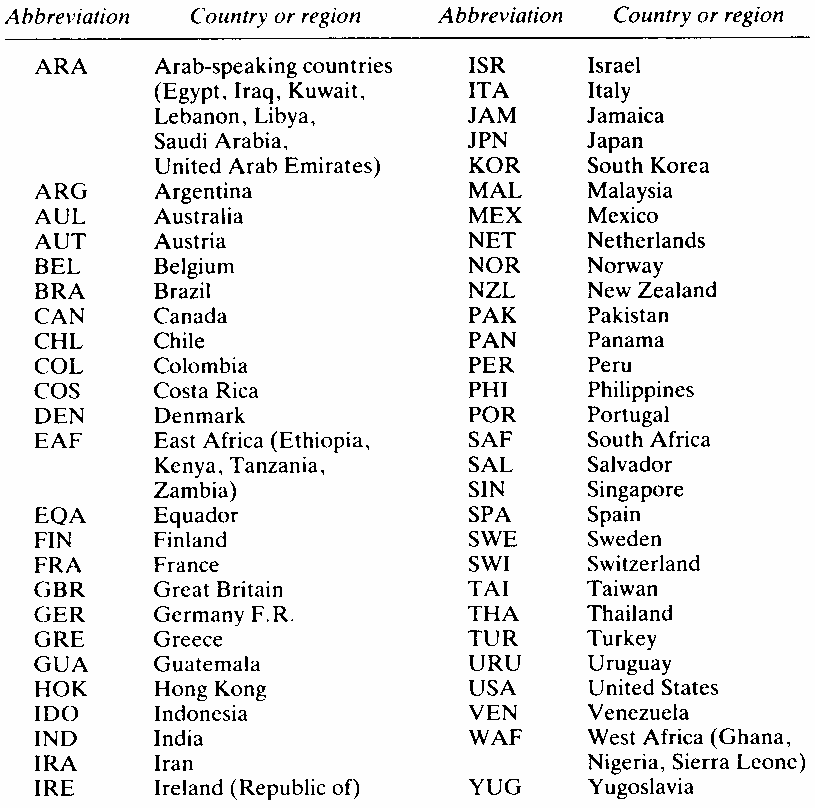
\includegraphics[width=0.65\linewidth]{hofstede_abbr.png}
	    \caption{Abréviations pour les pays et régions étudiés}
	   \end{center}
	  \end{figure}
	  
	  \begin{figure}[!ht]
	   \begin{center}
	    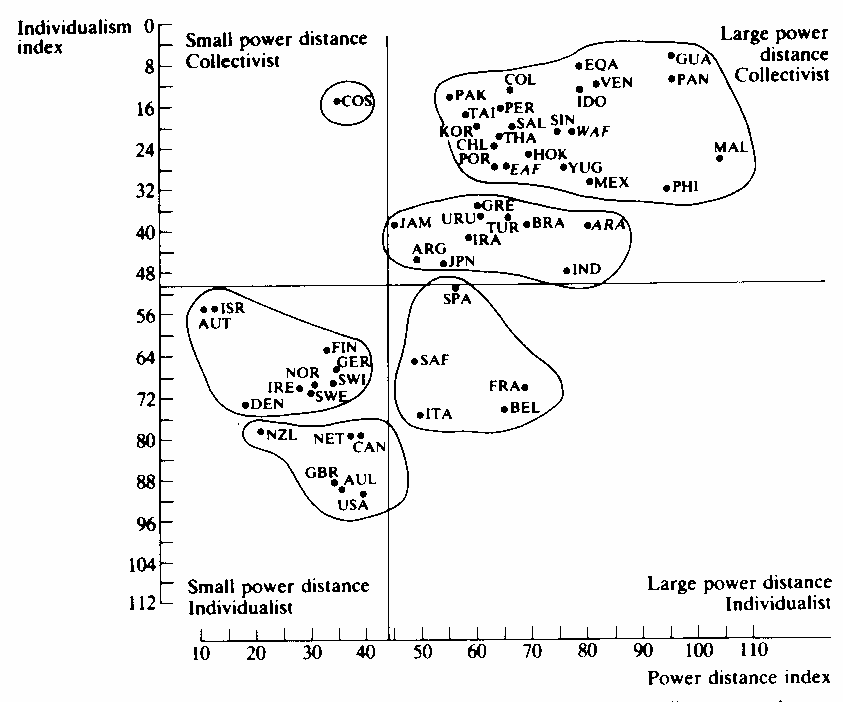
\includegraphics[width=0.65\linewidth]{hofstede_indivi_collect.png}
	    \caption{Position des 50 pays et 3 régions sur la distance au pouvoir et l'individualisme-collectivisme}
	   \end{center}
	  \end{figure}
	  
	  \begin{figure}[!ht]
	   \begin{center}
	     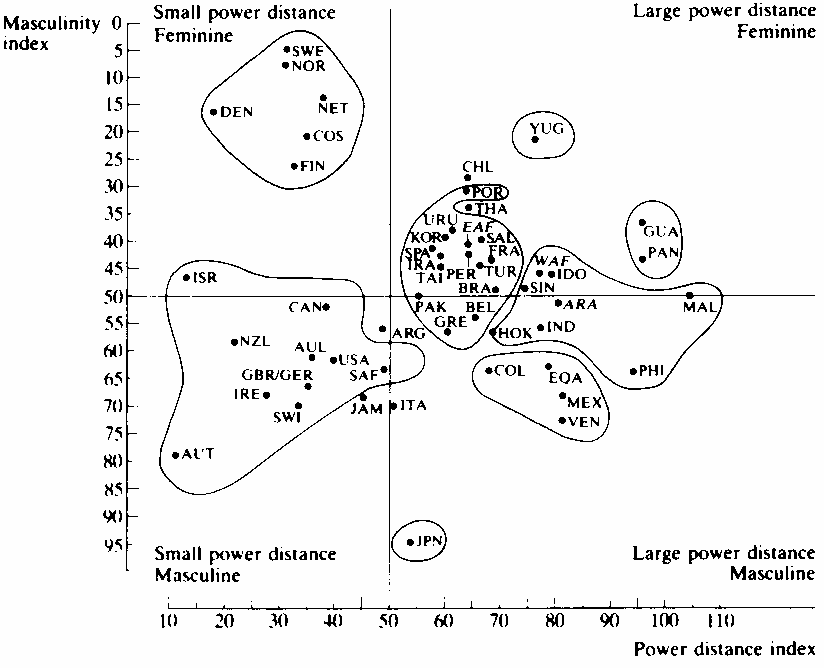
\includegraphics[width=0.65\linewidth]{hofstede_power_masc.png}
	     \caption{Distance au pouvoir contre masculinité pour 50 pays et 3 régions}
	   \end{center}
	  \end{figure}

	  \begin{figure}[!ht]
	   \begin{center}
	     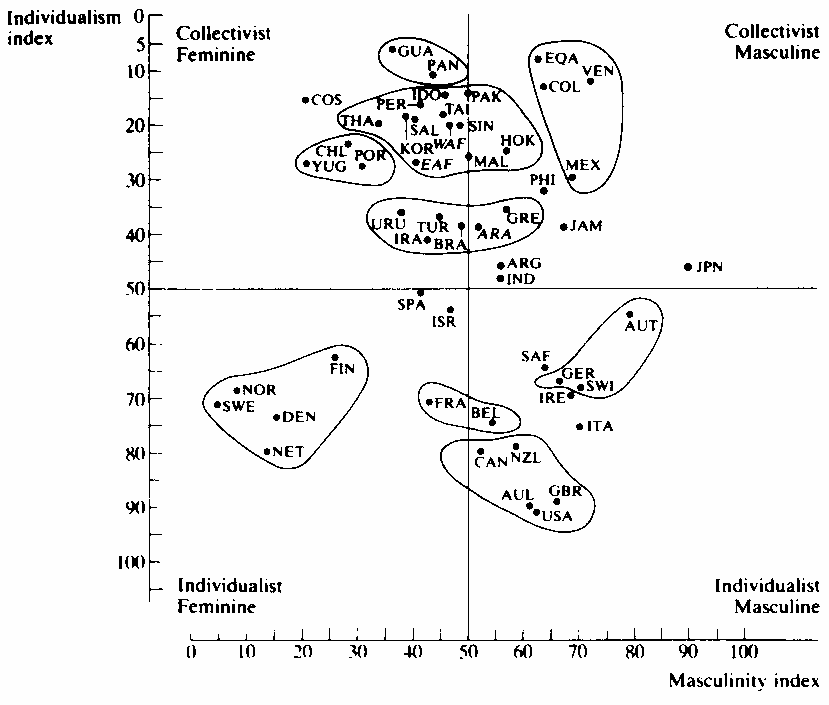
\includegraphics[width=0.65\linewidth]{hofstede_masc_indivi.png}
	     \caption{Position de 50 pays et 3 régions sur les dimensions masculinité-féminité et individualisme-collectivisme}
	   \end{center}
	  \end{figure}
	  
	  \begin{figure}[!ht]
	   \begin{center}
	    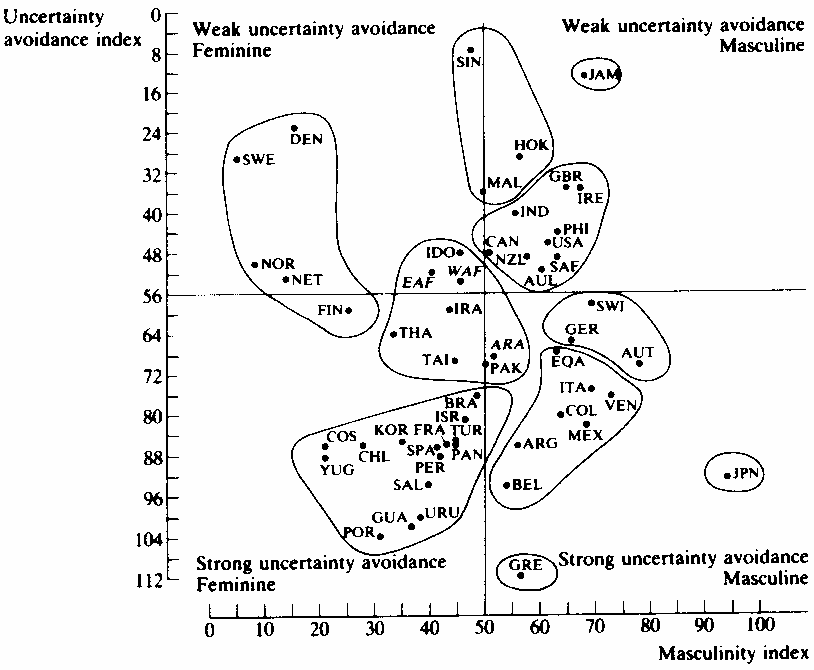
\includegraphics[width=0.65\linewidth]{hofstede_masc_incertitudes.png}
	    \caption{Position de 50 pays et 3 régions sur les dimensions masculinité/féminité et évitement de l'incertitude}
	   \end{center}
	  \end{figure}
	  
	  \begin{figure}[!ht]
	   \begin{center}
	    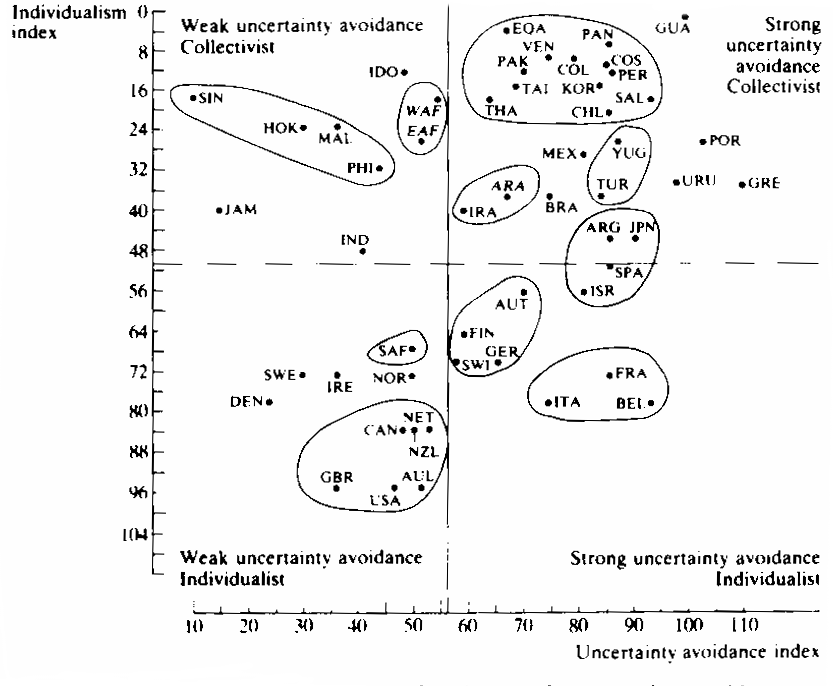
\includegraphics[width=0.65\linewidth]{hofstede_incertitudes_indivi.png}
	    \caption{Position de 50 pays et 3 régions sur les dimensions d'évitement d'incertitude et individualisme-collectivisme}
	   \end{center}
	  \end{figure}

	  \FloatBarrier % Force les flottants à se placer ici


	\subsection{Le cycle de perpétuation culturelle (Sathé, 1985)}
		\subsubsection{Un phénomène dynamique}
		
		\begin{figure}[h]
			\begin{center}
			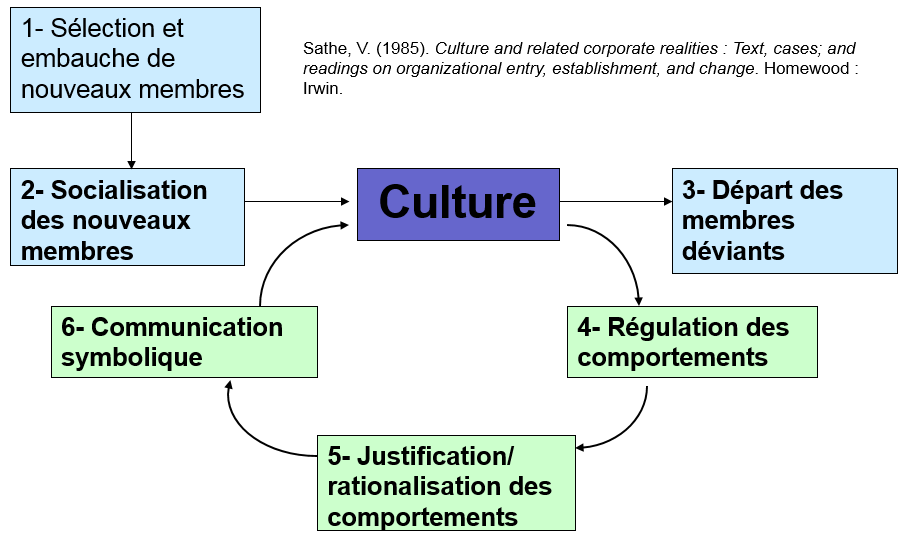
\includegraphics[scale=0.5]{modele_sathe.png}
			\caption{Cycle de perpétuation culturelle de Sathé}
			\label{modele_sathe}
			\end{center}
		\end{figure}
		
		L'entreprise dispose de plusieurs moyens pour faire perpétuer sa culture ou bien la renouveler (fig.~\ref{modele_sathe}).
		\begin{enumerate}
		\item Le candidat choisit une entreprise correspondant à ses valeurs. Et ceci va dans l'autre sens aussi, une entreprise n'accepte que les candidats correspondants à ses valeurs ou juger capable d'y adhérer.
		\item Le candidat accepté devra alors intégrer de nouvelles normes, valeurs, comportements propres à la culture de l'entreprise.
		\item Les membres qui n'adhèrent pas à la culture d'entreprise quittent cette dernière.
		\item Dans cette étape, l'entreprise vérifie, à l'aide de grilles d'évaluations, si le comportement d'un employé est bénéfique pour elle. Un comportement considéré comme favorable sera encouragé.
		\item On travaille entre l'adéquation culturelle entre chaque membre et l'entreprise. \newline
		ex:  Je fais ça par objectif, ou bien je fais ça pour que l'entreprise perdure même si mon acte n'est pas moral.
		\item Différents moyen de communication sont utilisé pour promouvoir la culture de l'entreprise. \newline
		ex: histoires, jargons, métaphores, logo, etc. \newline
		\end{enumerate}
		
		Il existe \textbf{3 leviers d'action pour agir sur la culture}:
		\begin{enumerate}
		\item Régulation des comportements.
		\item Rationalisation des comportements.
		\item Communication symbolique.
		\end{enumerate}
		
	\subsection{Les composantes de la culture organisationnelle (Thévenet)}
	
	La culture d'entreprise est la combinaison de différents matériaux culturels, chacun ayant des caractéristiques propres (Fig.~\ref{thevenet}).
	
	\begin{figure}[h]
	   \begin{center}
	    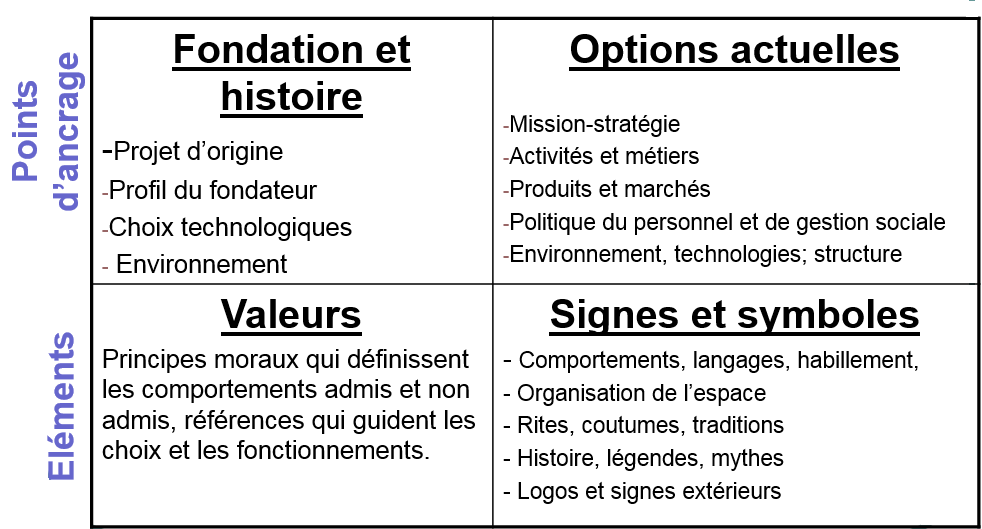
\includegraphics[width=0.65\linewidth]{thevenet.png}
	    \caption{Modèle de Thévenet}
	    \label{thevenet}
	   \end{center}
	  \end{figure}
	
	
	\subsection{Méthodologies d'étude}
		%TODO rechercher plus d'informations
		L'entreprise \textbf{EST une culture} : approches qualitatives, idiosyncrasiques, cliniques et ethnographiques. Ceci correspond au côté non conscient de Schein.\newline
		
		L'entreprise \textbf{A une culture} : approches quantitatives, nomothétiques, par questionnaires. Ceci correspond au côté artefact de Schein. \newline
		
		Il y a 2 mécanismes sous-jacents:
		\begin{itemize}
		\item Favoriser l'intégration interne.
		\item Aider les gens à s'adapter à l'environnement. \newline
		\end{itemize}
		
		Il y a 2 questions:
		\begin{itemize}
		\item Certains types de culture sont-ils associés à une meilleure performance?
		\item Une entreprise est-elle plus performante si elle est a une culture « forte »?
		\end{itemize}

		\subsubsection{Type de culture et performance}
		
		Il existe plusieurs études empiriques liant la performance avec un type de culture. Voici quelques exemples:
		\begin{itemize}
		\item Denison (1990): Effet bénéfique des pratiques de management participatives et d'une bonne organisation du travail.
		\item Gordon \& Di Tomaso (1992): Dans le secteur des assurances, l'adaptabilité est plus profitable que la stabilité.
		\item Calori \& Sarnin (1991): Taux de croissance de l'entreprise lié à un orientation vers les personnes et vers le changement. \newline
		\end{itemize}
		
		\begin{figure}[h]
			\begin{center}
			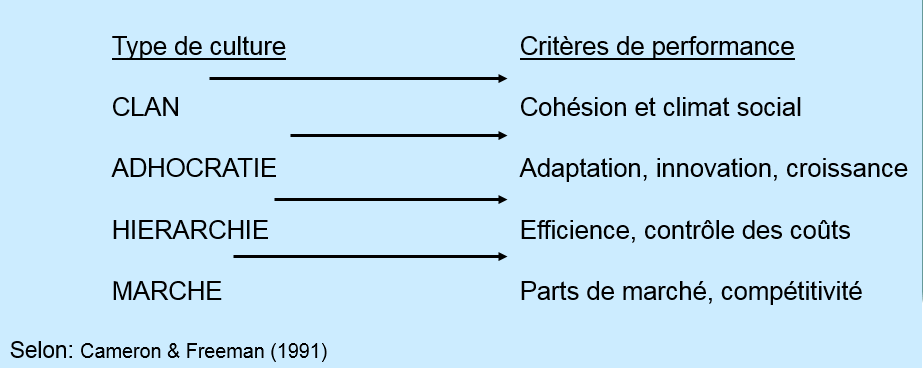
\includegraphics[scale=0.5]{culture_performance.png}
			\label{culture_performance}
			\caption{Type de culture et perfomance (Cameron \& Freeman, 1991)}
			\end{center}
		\end{figure}
		
		Mais cependant, de ces expériences, aucun résultats ne convergent car \textbf{la performance est un construit multidimensionnel et contingent} (fig.~\ref{culture_performance}). \newline
		ex: La culture adhocratique favorise la performance en termes d'innovation.
		
		\subsubsection{Culture et réactions individuelles}
		
		La culture a un triple rôles: 
		\begin{itemize}
		\item Affectif: identification à l'entreprise.
		\item Cognitif: réduction de l'incertitude.
		\item Comportemental: pression sociale. \newline
		\end{itemize}
	
		2 questions:
		\begin{itemize}
		\item Les différents types de culture sont-ils associés à des comportements spécifiques?
		\item Quelle est l'influence de l'adéquation individu-organisation?
		\end{itemize}

		\subsubsection*{Type de culture et réactions individuelles}
		
		La figure ~\ref{type_culture_reactions_individuelles} reprend les différents types de culture et les réactions individuelles qui peuvent en découler.
		
		\begin{figure}[h]
			\begin{center}
			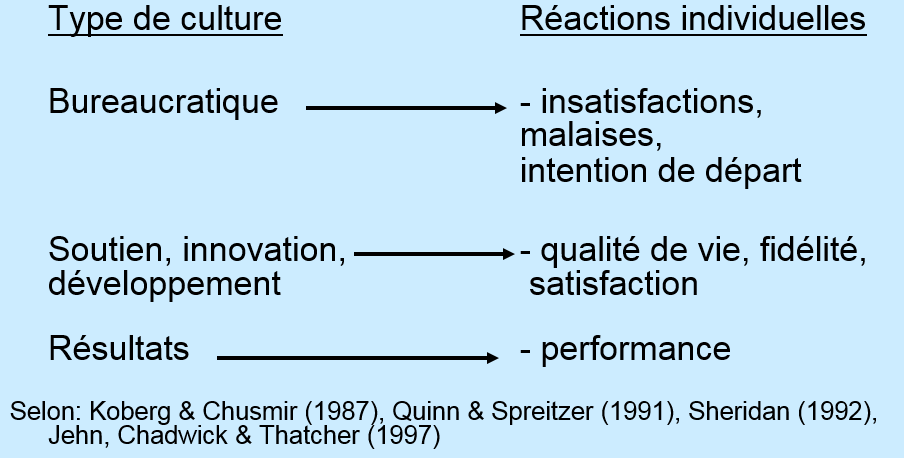
\includegraphics[scale=0.5]{type_culture_reactions_individuelles.png}
			\caption{Type de culture et réactions individuelles.}
			\label{type_culture_reactions_individuelles}
			\end{center}
		\end{figure}				
		
		\subsubsection*{Adéquation individu-organisation et réactions individuelles}
		
		\begin{figure}[h]
			\begin{center}
			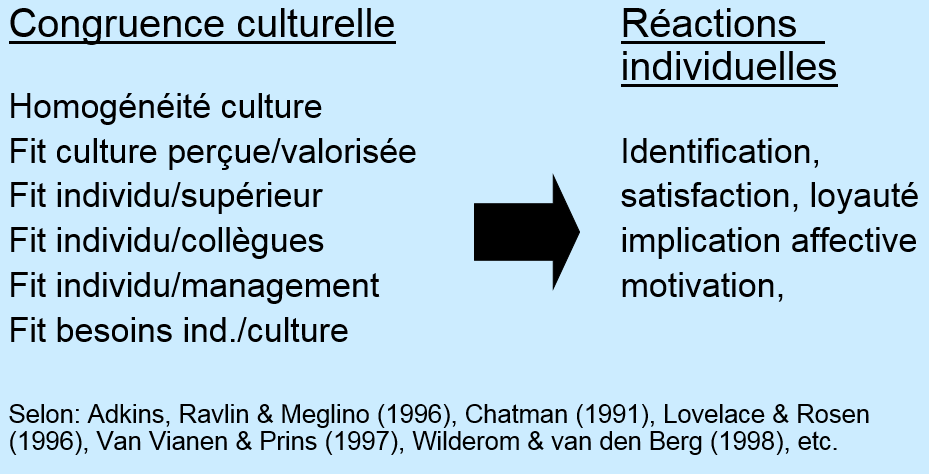
\includegraphics[scale=0.5]{adequation_individu-organisation_reactions_individuelles.png}
			\caption{Adéquation individu-organisation et réactions individuelles.}
			\label{adequation_individu-organisation_reactions_individuelles}
			\end{center}
		\end{figure}			
		
		\subsubsection{Conclusion}
		
		La culture organisationnelle: 
		\begin{itemize}
		\item Une construction sociale, fruit des interactions symboliques entre acteurs, 
		\item Dont la cohésion (homogénéité) importe plus que les orientations (types), 
		\item Repère affectif, cognitif et comportemental pour les membres de l'organisation, 
		\item Levier de coordination et de mobilisation pour l'entreprise, 
		\item Facteur de stabilité et d'inertie, voire frein à l'innovation et à l'adaptation. 
		\end{itemize}
		
\section{Dynamique de groupe}
	\subsection{Le groupe dans l’histoire de l’organisation}
	
	La vision qu'on s'est faite du groupe a fortement évolué dans le temps: \newline
	
	Dans l'\textbf{Organisation Scientifique du Travail}, le groupe était perçu comme quelque chose de nuisible par le manager. Le but du Taylorisme est d'atomiser les groupes pour qu'ils n'existent pas. Les groupes formés étaient soit informel, soit alors clandestin. Cette vision perdure jusqu'à l'École des Relations Humaines.\newline
	
	Avec l'\textbf{École des Relations Humaines}, on remarque que le groupe peut avoir des effets bénéfiques. On commence à s'intéresser au bien-être qui impacte fortement l'efficacité. On considère le groupe comme quelque chose de positif. Il est conçu comme une source d'appartenance, de motivation et de conformisme.\newline
	
	Puis vient le \textbf{Courant Socio-Technique} avec qui on remarque que les changements techniques peuvent avoir de graves conséquences sur les relations humaines. L'équipe est alors très importante pour le changement.\newline
	
	Et enfin arrive l'\textbf{Entreprise Flexible} qui se caractérise par une gestion plus flexible des équipes. On met ensemble des experts pour travailler sur un projet (équipes projets ad hoc).
	
	\subsection{Définitions et types}
		\subsubsection{Définition}
		
		Le \textbf{groupe} est un \textit{ensemble} de 2 individus ou plus, \textit{interdépendants} dans la poursuite d'un \textit{but} identique. \newline
		
		Il est caractérisé par:
		\begin{itemize}
		\item Système social perçu comme une entité: il y une frontière entre les membres et les non-membres.
		\item Système social structuré et différencié: mécanisme de coordination.
		\item Interdépendance dans la réalisation d'une ou plusieurs tâches: certaines tâches ne sont pas réalisables sans les autres membres du groupe.
		\item Système ouvert sur son environnement: l'environnement (personnes en dehors du groupe) a un impact sur le travail du groupe.
		\end{itemize}
		
		\subsubsection{Types}
		
		On peut distinguer les groupes selon leur \textit{objectif} et la façon dont les \textit{interdépendances} sont structurés.	A partir de cela, on obtient 2 groupes: \newline
		
		Le \textbf{groupe informel} qui n'a pas de structure formellement définie par l'organisation. Ces groupes ne sont pas négligeables. C'est à l'intérieur de ces groupes que se transmettent les rumeurs,... De plus, s'ils ne sont composés d'aucun employés travaillant ensemble, on peut supposer qu'il y a des soucis (surtout vrai pour les groupes d'affinités). Le groupe informel peut lui-même être subdivisé en 2 catégories:
		\begin{itemize}
		\item \textbf{Groupe d'affinité} qui sont des personnes se réunissant pour partager un ou plusieurs points communs.\newline 
		ex:Personnes qui courent ensemble.
		\item \textbf{Groupe d'intérêt} qui sont des personnes travaillant ensemble pour atteindre un objectif spécifique.\newline 
		ex:Employés qui se rassemblent pour une pétition suite au licenciement d'un collègue. \newline
		\end{itemize}
		
		Le \textbf{groupe formel} est un groupe de travail déterminé par la structure de l'entreprise. Le groupe formel peut lui aussi être subdivisé en 2 catégories:
		\begin{itemize}
		\item Le \textbf{groupe hiérarchique} est groupe composé d'individus qui se réfèrent directement à un responsable déterminé.
		\item Le \textbf{groupe de travail} est un ensemble de personnes travaillant ensemble afin de réaliser une tâche ou un projet spécifique. Dans ce type de groupe de travail, on ne se réfère pas forcément à un supérieur. Il est possible d'en choisir un pour le projet seulement.\newline
		ex: Parents, professeurs et le directeur qui se réunissent pour discuter de l'expulsion d'un élève. Chaque personne emmène son expertise. Il n'y a pas de vrai hiérarchie. \newline
		\end{itemize}
		
		On peut aussi diviser les équipes de travail selon l'\textit{empowerment} ( dans quelle mesure les équipes disposent de pouvoir pour se strucuture):
		\begin{itemize}
		\item \textbf{Traditionnelles} qui est sous la direction d'un supérieur (organigramme).
		\item \textbf{Consultatives} dont les membres de l'équipe peuvent proposer des solutions mais la décision finale revient au chef. \newline
		ex: Cercles de qualité.
		\item \textbf{Ad hoc} qui sont des groupes de projets ponctuels. Ils disposent d'une marge de man\oe{}uvre pour leur structuration.
		\item \textbf{Semi-autonomes} qui sont des équipes de travail ayant un but de production mais disposant d'une liberté de gestion. 
		\end{itemize}
		
		
	\subsection{Dynamique des groupes restreints}
	
	Un \textbf{groupe restreint} est un groupe disposant d'un nombre de membres réduit (inférieur à 20). \newline
	
	La \textbf{dynamique de groupe} est l'ensemble des phénomènes, mécanismes et processus psychiques et sociologiques qui émergent et se développent dans les petits groupes sociaux.
	
		\subsubsection{Anzieu et Martin (1968)}
		%TODO 
		
		\subsubsection{Les étapes de la vie d’un groupe (Tuckman, 1965)}
		
		Les groupes se constituent. Ils passent par différentes étapes : \newline
		%Film "Remember the titans"
		\begin{itemize}
		\item \textbf{Formation} (ou constitution): durant cette étape on travaille la \textit{confiance}. On ne connaît pas les autres membres du groupe, leurs normes, .... On essaye dès lors d'observer comment le groupe agit mais en gardant une certaine distance. On est en pleine incertitude. Cette étape se termine quand on sent qu'on appartient au groupe.
		\item \textbf{Agitation}: c'est l'étape de \textit{structuration des tâches et des rôles} (pas simple et parfois lente). Il faut définir une hiérarchie. Cette période est également caractérisée par des conflits. Cette phase est importante et incontournable.
		\item \textbf{Normalisation}: on crée des \textit{normes} de fonctionnement et chaque membre doit y \textit{adhérer}. Les liens se renforcent. Il y a un sentiment d'appartenance. Cette étape se termine quand tout le monde sait comment se comporter.
		\item \textbf{Performance} (ou rendement): on se concentre sur la performance. Réalisation des buts et adaptation.
		\item \textbf{Dissolution}: fin du groupe. Peut être difficile pour certaines personnes. \newline
		\end{itemize}
		
		On peut toutefois porter certaines critiquer sur le modèle. En effet, le modèle est \textit{linéaire}. Tuckman suppose qu'on ne peut pas revenir à une étape antérieure. De plus, il ne tient pas compte du \textit{contexte} ou de l'\textit{environnement}. Dés fois, on doit être performant tout de suite ou bien certaines étapes sont faites à votre place (chef, normes, ... définis déjà par l'organisation par exemple). \newline
		
		On a remarqué que ces groupes se remettent en question au même moment.\newline
		%TODO schéma montrant performance en fonction du temps		
		
		Il existe aussi une dynamique des \textbf{groupes temporaires}.\newline
		ex: Un groupe formé pour 2h seulement. \newline
		
				
		\subsubsection{Cohésion affective}
		
		La \textbf{cohésion affective} est le degré d'\textit{attractivité} des membres les uns pour les autres. \newline
		
		Elle est fonction de l'\textit{homogénéité} du groupe. Un groupe composé de personnes similaires ayant plusieurs points communs aura une meilleure cohésion. Elle accroît la \textit{satisfaction} et renforce le \textit{conformisme}. Toutefois, la cohésion affective est \textbf{faiblement corrélé à la performance}. Une grande cohésion peut emmener tout les membres du groupe à prendre la même décision qui est la mauvaise. \newline
		
		On peut analyser la cohésion affective d'un groupe ou organisation à l'aide d'un \textbf{sociogramme}. \newline 
		
		Un sociogramme est un diagramme des liens sociaux qu'une personne possède. Les critères qui servent à établir un tel diagramme sont divers: relations personnelles, relations professionnelles, canaux de communication, .... Cet outil permet d'objectiver la dynamique des groupes, afin qu'un animateur ou un enseignant, par exemple, soient moins influencés par leurs sentiments et leurs préjugés lorsqu'ils établissent des équipes de travail.\newline
		%TODO schéma sociogramme
		
		
		\subsubsection{Facteurs de cohésion d’un groupe}
		Voir tableau ~\ref{facteurs_cohesion}.
		\begin{table}[htc]
	        \begin{tabular}{p{7cm}|p{7cm}}
		\textbf{Facteurs favorables} & \textbf{Facteurs défavorables} \\ 
		\hline \hline
		Homogénéité du groupe & Hétérogénéité du groupe \\ \hline
		Accord sur les buts du groupe & Désaccord sur les buts \\ \hline
		Menace externe & Aucune menace extérieurs \\ \hline
		Compétition intergroupes & Compétition intragroupe \\ \hline
		Taille réduite & Grande taille \\ \hline
		Succès, attraction personnelle & Echec, expérience désagréable \\ \hline
		Fréquence des interactions & Peu d'interactions \\ \hline
		Bonne communication & Mauvaise communication \\ \hline
		Faible turn over & Turn over élevé \\ \hline
		Evaluation favorable & Domination par un ou plusieurs membres \\ \hline
	    \end{tabular}
	    \caption{Facteurs de cohésion d'un groupe.}
	    \label{facteurs_cohesion}
	  \end{table}
		
				
		\subsubsection{Structuration des rôles et statuts}
		
		Les \textbf{rôles} sont un ensemble d'attitudes et comportements attendus de celui qui occupe une position dans un groupe. \newline 
		%TODO trouver une meilleure phrase
		Plusieurs catégories par rapport au rôle:
		\begin{itemize}
		\item \textbf{Attentes de rôles}: du fait qu'on occupe un rôle bien déterminé, les autres membres (ou même des extérieures au groupe) peuvent avoir certaines attentes par rapport à toi. Parfois des attentes non fondées. Il y a donc risque de conflits et d'ambiguïtés de rôles.
		\item \textbf{Identité de rôle}: attitudes et comportements attendus du rôle. On peut changer aussi de rôle, identités multiples qui sont parfois conflictuelles. C'est la vision que se font les autres du rôles.
		\item \textbf{Perception de rôle}: idée qu'on se fait des attitudes et comportements à prendre du rôle qu'on occupe. Il y a risque de décalage entre attentes et perceptions. C'est la vision que moi, qui occupe le rôle, se fait justement de ce rôle. \newline
		\end{itemize}
		
		%TODO ajouter lien youtube.
		On peut illustrer la notion de rôle par l'\textbf{expérience de Zimbardo}(1971).C'est une étude  de  psychologie  expérimentale  sur  les  effets  de  la  situation  carcérale. Des  étudiants 
(sélectionnés  pour  leur  stabilité  et  leur  maturité) jouent  aléatoirement  le  rôle  de  gardiens  ou  de 
prisonniers. Cette expérience vise l’étude du comportement de personnes ordinaires dans un tel contexte, l’étude 
eut pour effet de montrer que c’est la \textbf{situation plutôt que la personnalité des participants qui était 
à l’origine de comportements parfois à l’opposé des valeurs professées par les participants avant 
l’étude}. Les étudiants agissent en fonction de leur rôle et non en fonction de leurs croyances. \newline

		Le \textbf{statut} est un ensemble d'attributs liés à la position d'un individu dans un système culturel donné. \newline
		
		On peut aussi définir le \textbf{statut} comme étant la place ou le rang occupé au sein d'un groupe et conférant un certain prestige.\newline
		
		Il existe \textbf{3} sources de statut. La première source est le \textbf{pouvoir exercé sur les autres}.	 La deuxième est la \textbf{capacité à contribuer aux objectifs du groupe}. Enfin, les dernières sont les \textbf{singularités propres à l'individu, valorisées par les groupe et le système culturel}. \newline
		
		Tout ceci influence le conformisme, les interactions et le sentiment d'équité. Une personne qui se conforme moins aux normes dispose souvent d'un statut plus élevé. De même, le fait de couper la paroles, se faire grand, ... sont les signes de quelqu'un qui occupe un statut privilégié (même si cela peut être négatif).
		
		\subsubsection*{Les 9 rôles d'équipiers de Belbin(1988)}		
		
		
		%Source belbinfrance.com		
		La \textbf{méthode Belbin} est un outil rationnel et rigoureux qui permet d'évaluer, de manière non intuitive, la coopération des membres d'une équipe. En identifiant les rôles endossés par chacun, on peut augmenter l'efficacité  des équipes en jouant, à bon escient , sur sa composition ou sur son fonctionnement interne.Il existe 9 rôles réparties en 3 catégories.\newline
		
		La \textbf{molécule de Belbin} illustre parfaitement le fait que les rôles se complémentent et que chaque rôle doit être présent dans l'équipe. \newline
		%TODO ajouter les schémas.
		\subsubsection{Normes, valeurs et conformisme}
		 Tout les groupes établissent des \textbf{normes}. Ces normes dictent ce que les membres peuvent, ne doivent pas faire, leur comportement attendu. C'est le principe de \textbf{normalisation}. \newline
		 
		 Le \textbf{conformisme} est le fait justement de s'ajuster à ses normes en adaptant son comportement. \newline
		 
		 Les gens se conforment aux normes du groupe le plus important auquel ils appartiennent ou souhaitent appartenir. Ces groupes principaux sont appelés \textbf{groupes de référence}.
		 
		 \subsubsection*{2 expériences princeps}
		 
		 \textbf{1. Années 30: Sherif et l'effet auto-cinétique.} \newline
		 
		 Pour étudier le principe de normalisation, Sherif utilise l'effet auto-cinétique qui est une illusion par laquelle un faible point lumineux semble se mouvoir (dans une pièce noir).  L'expérience consistait à indiquer la distance dont le point s'est déplacée. L'expérience s'est déroulé en 2 étapes. \newline
		 
		 Dans la première étape, les sujets passaient chacun à leur tour l'expérience. Les résultats, à ce moment varie d'une personne à l'autre. \newline
		 
		 Dans la deuxième étape par contre, les sujets étaient rassemblés en groupe et passaient l'expérience ensemble.  Les résultats, à ce moment sont identiques. Les sujets se sont mis d'accord sur une réponse commune. Ils ont établis une norme. \newline
		 
		 La conclusion de l'expérience est alors que chaque groupe établit des normes, c'est-à-dire des comportements standards adoptés par leurs membres. \newline
		 
		 \textbf{2. Années 50: l'effet d'Asch.}\footnote{\url{https://www.youtube.com/watch?v=MBQ_nGy8tMk}} \newline
		 
		 Asch a étudié l'impact de la pression exercée par les groupes pour faire plier les membres à une certaine conformité. \newline
		 
		 L'expérience consiste à placer une poignée d'individus derrière une table, visionnant des cartes montrant 3 barres de taille différente. Chaque individu, tour à tour, doit dire laquelle des 3 barres a la même longueur qu'une autre barre que l'on leur présente. La subtilité : il n'y a qu'un seul individu qui réalise effectivement l'expérience, les autres étant des complices qui répondent incorrectement. \newline
		 
	Les résultats montrent que, par peur d'opposition aux inconnus du groupe, l'individu répond la même mauvaise réponse que les autres. Le caractère inconnu des membres du groupe est important. Lorsque ce sont des personnes connues, le conformisme est moindre. Lorsque l'un des inconnus répond autrement que les autres, le conformisme est moindre, et ce, même si cette autre minorité ne répond toujours pas correctement. \newline
	
	La conclusion de cette expérience est que le conformisme est \textbf{indépendant de la taille du groupe}, \textbf{réduit si autre avis minoritaire} et \textbf{accru si forte cohésion du groupe}. \newline
	
	Il y a 2 ressorts du conformisme. La première est la \textbf{dépendance informationnelle} (besoin de certitude). La deuxième est la \textbf{dépendance normative} (besoin d'approbation). \newline
	
	A noter que \textbf{groupe d'appartenance} n'est pas la même chose que  \textbf{groupe de référence}. Le groupe d'appartenance correspond au groupe d'origine, ancré dans le passé. Tandis que le groupe de référence est lui tourné vers le futur, c'est le groupe auquel on aspire. \newline
	
	En conclusion, tout groupe est créateur de normes propres de performance, d'appartenance, d'interactions sociales ou/et d'attribution de ressources. Et tout groupe exerce une pression au conformisme, ce qui rend  les normes particulièrement résistantes au changement. 
		 		
		\subsubsection{La pensée de groupe (Janis, 1972)}
		
		La pensée de groupe c'est la tendance des membres, dans un groupe à forte cohésion, à dissimuler une opinion divergente ou minoritaire, voire à perdre tout sens critique sous la pression des normes de conformité.  \newline
		\og{}\textit{Ce n'est pas parce qu'ils sont plus à avoir tort qu'ils ont raison.}\fg{} (Coluche) \newline
		
		Symptômes de la pensée de groupe:
		\begin{itemize}
		\item Cohésion forte et pressions sur les individus dissidents.
		\item Illusion partagée d'unanimité et d'exactitude.
		\item Ignorance et déni des signaux contraires (auto-censure).
		\item Fermeture à l'information provenant de l'extérieur du groupe.
		\item Stéréotypisation et ridiculisation des groupes extérieurs. \newline
		\end{itemize}
		
		Conditions propices:
		\begin{itemize}
		\item Préoccupation pour la cohésion du groupe.
		\item \og{}Insularisation\fg{}, isolement du groupe.
		\item Décision dans l'urgence, sous stress.
		\item Décision dans analyse systématique des alternatives possibles, absence de méthode.
		\item Groupe dominé par un individu, leadership directif. \newline
		\end{itemize}
		
		Techniques évitant la pensée groupale:
		\begin{itemize}
		\item \textbf{Remue-méninges} (brainstorming):Cette technique consiste à encourager l'émission de toutes les idées novatrices possibles, sans en autoriser la critique. Le fait qu'une idée en engendre une autre et que les jugements ne soient pas permis encourage les membres à laisser libre court à leur imagination.
		\item \textbf{Avocat du diable}: quequ'un qui va systématiques poser des objections aux idées avancées.
		\item \textbf{Groupe nominal}: La  technique  du  groupe  nominal  est une  approche  de  brainstorming  plus  structurée, appelée "nominale" car, au cours de la session, le groupe n'atteint pas le niveau habituel d'interaction propre à une véritable équipe. C'est un outil efficace à utiliser lorsque certains membres ou tous les membres du groupe ne se connaissent pas encore.
		\end{itemize}
		
	\subsection{Le groupe, levier de changement}
	
	\subsubsection*{1943: Etude de Kurt Lewin sur la consommation d'abats.}
	
	Durant la guerre, les autorités cherchent à convaincre les ménagères de faire consommer des abats de b\oe ufs à leurs familles pour préserver les beaux morceaux pour les soldats. \newline
	
	L'expérience de Lewin consistait en 6 groupes de 13 à 17 ménagères à propos des produits de consommation. \newline
	
	Ces ménagères ont été soumises soit à un exposé de 45 minutes (3\% de changement d'habitudes), soit à une discussion de groupe avec nutritionnistes (32\% de changement d'habitudes). \newline
	
	Suite à l'expérience de Lewin, on  peut  dire  que l'implication  par  la  discussion  est  supérieure  à l'écoute  d'un  exposé.  Elle  permet  la  modification  des  habitudes  et  réduit  la  résistance  au changement. De plus le petit groupe atteint davantage l'individu qu'une communication de masse. \newline
	
	Le groupe est donc un puissant levier de changement des normes sociales mais aussi un champ de forces motrices et restrictives en équilibre quasi-stationnaire. \newline
	%TODO RESEARCH CENTER FOR GROUP DYNAMICS MICHICHANG
	
	\subsubsection*{Le champ de forces quasi-stationnaire de Lewin.}
	
	\begin{figure}[h]
		\begin{center}
		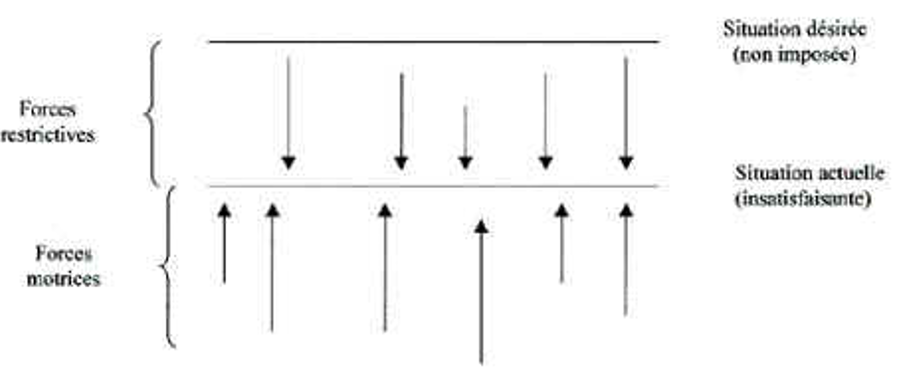
\includegraphics[scale=0.50]{champ_forces_lewin.png}
		\caption{Champs de forces quasi-stationnaire de Lewin.}
		\end{center}
	\end{figure}
	
	Pour Lewin, les actes d'une personne ne sont pas stables, linéaires. Il y a des forces motrices et des forces restrictives qui influencent nos comportements. Pour changer un comportement, il faut non pas toucher aux forces motrices mais plutôt lever toutes les forces restrictives.
	
	ex: Aller au cours.
	\begin{itemize}
	\item Forces motrices: c'est plus facile pour étudier, comprendre, ...
	\item Forces restrictives: il faut se lever tôt, on ne peut pas sortir la veille,... 
	\end{itemize}
	
	\subsubsection*{Les 3 phases de changement.}
	
	\begin{figure}[h]
		\begin{center}
		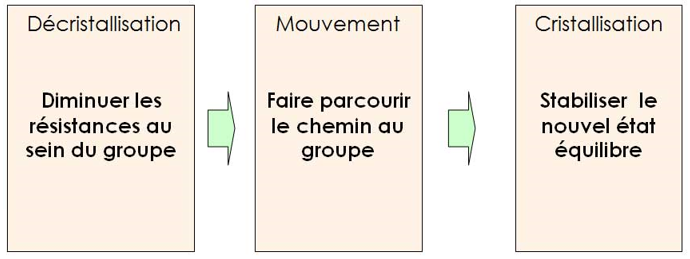
\includegraphics[scale=0.50]{phases_changement_lewin.png}
		\caption{Les 3 phases du changement de Lewin.}
		\end{center}
	\end{figure}
	
	Ce sont:
	\begin{enumerate}
	\item \textbf{Décristallisation}, dégel: déstabilisation du champ de forces.
	\item \textbf{Changement}, évolution des normes et comportements.
	\item \textbf{Recristalisation}, stabilisation du champ de forces.
	\end{enumerate}
	
	\subsubsection*{La méthode de la recherche-action.}
	
	C'est une méthode planifiée et participative visant un double objectif de changement concret dans le système et de production de connaissances sur celui-ci.
	\begin{enumerate}
	\item Identification du problème.
	\item Collecte des données.
	\item Feed-back des données au groupe visé.
	\item Diagnostic.
	\item Action.
	\item Evaluation. \newline
	\end{enumerate}
	
	L'acteur  devient  chercheur  et  le  chercheur  est  immanquablement  acteur. En effet, lorsque le chercheur va observer une civilisation par exemple, il influence les comportements  de  celle-ci.  Il  devient  un  acteur  de  la  situation  qu'il  observe. \newline
	
	Refus  du  postulat  d'objectivité  du  positivisme  :  la  connaissance  n'est  ni  extérieure,  ni universelle  et  ni  objective  mais  est  dans  l'action,  la  subjectivé  en  contexte. La  recherche-action  ne  produit  donc  pas  de  connaissance  objective  mais  bien  toujours contextualisée.
	
	\subsubsection*{L'influence des minorités.}
	
	Une minorité est capable de changer la position de la majorité si elle dispose d'une \textbf{position stable et cohérente} et si elle \textbf{n'est pas considérée comme déviante}. \newline
	
	Ceci \textbf{accroît l'indépendance d'esprit et la pensée divergente}. Une majorité est plus créative si elle est exposée à une minorité proposant des alternatives. De plus, \textbf{la conversation est d'abord privée avant d'être publique}.
	
	\subsection{Entreprise flexible : l'équipe de travail, lieu d'efficacité}
	
	Chaque  entreprise,  comme  chaque  institution,  possède  sa  personnalité.  De  ses  composantes humaines, physiques et sociales émane un climat organisationnel qui lui est propre. Cet aspect de l'entreprise constitue un élément clé trop souvent mésestimé, voire ignoré. \newline
	
Luc  Brunet  et  André  Savoie  proposent  dans <<\textit{Le  climat  de  travail}>>(Montréal,  1999)  un  cadre  de  référence permettant une meilleure compréhension des dynamiques de l'individu, du groupe et de l'organisation. 
%TODO ajouter schéma 
	
	\subsubsection*{Critères d'efficacité des équipes de travail. (Savoie et Beaudin)}
	
	Voir figure ~\ref{criteres_efficacite_equipe}.
	\begin{figure}
		\begin{center}
		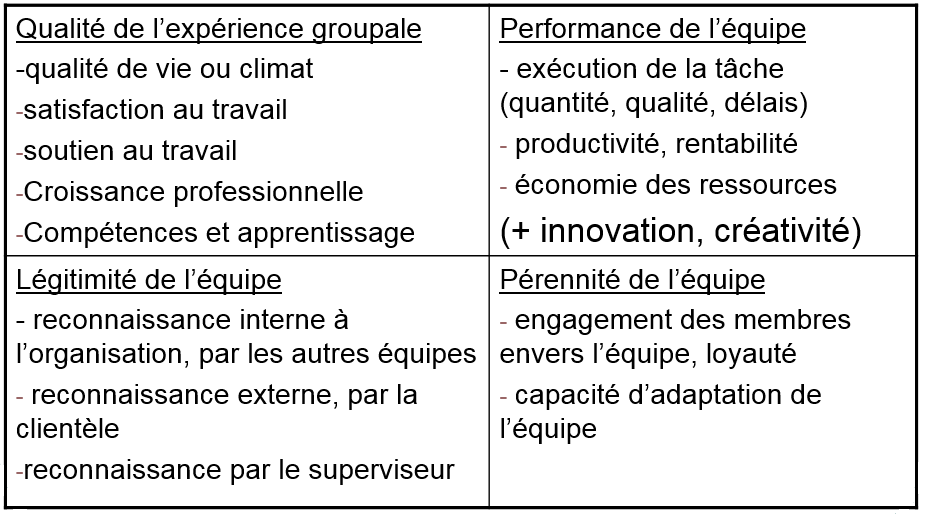
\includegraphics[scale=0.6]{criteres_efficacite_equipe.png}
		\caption{Critères d'efficacité des équipes de travail.}
		\label{criteres_efficacite_equipe}
		\end{center}
	\end{figure}
	
	\subsubsection*{Facteurs d'efficacité d'une équipe.}
	
	\begin{enumerate}
	\item Interdépendance de l'équipe envers l'environnement: orientation vers des buts externes, évaluation de son environnement, recherche de feed-back externes, coordination avec amont et aval.
	\item Interdépendance des équipiers: interdépendance structurelle dans l'organisation et la réalisation des tâches, pris de décision collective, feed-back et récompense d'équipe.
	\item Qualité des transactions entre équipiers: interdépendance affective et solidarité, qualité des relations, communications et interactions.
	\item Composition de l'équipe: équilibre entre homogénéïté (compatibilité des valeurs, …) et hétérogénéïté (complémentarité des compétences, …), taille et ratio membres/ tâches.
	\end{enumerate}
	
	\subsubsection*{Caractéristiques d'une équipe performante.}
	
	\begin{enumerate}
	\item  Sentiment d'avoir un but commun: mandat clair et stimulant, adhésion aux objectifs.
	\item Pouvoir d'agir avec autorité (empowerment): habilitation à prendre des décisions, gérer les ressources et les tâches, définir ses processus et façons de faire, être responsable des résultats.
	\item Profil et interdépendance des équipiers: compétences, engagement, coopération, échange et réciprocité.
	\item Ouverture de la communication: : écoute, dialogue et débat, reconnaissance et confiance mutuelles.
	\item Reconnaissance et appréciation: système de récompense, reconnaissance des contributions, considération par le supérieur.
	\end{enumerate}
	
	\subsubsection*{Le fonctionnement interne des équipes efficaces. (Aubé et Rousseau)}
	
	%TODO ajouter schéma productif et contre productif	
	
	\subsubsection*{Les interventions régulatrices groupales. (Aubé et Rousseau)}
		
	Se donner des objectifs communs, avoir un feed-back collectif et jouer sur les récompenses de groupe facilitent le fonctionnement de groupe. \newline
	
	Ces mécanismes ont un effet sur trois variables médiatrices, qui sont autant de composantes d'un groupe efficace. Les stratégies adoptées, les efforts fournis et la coopération. \newline
	
	Le  degré  d'interdépendance  des  équipiers  est  la  variable  modératrice. Autrement dit, tous les facteurs précités sont d'autant plus importants que les coéquipiers sont interdépendants.
	%TODO ajouter schéma	
	
	
	\subsubsection*{Pratiques de gestion des groupes à privilégier et éviter. (Aubé et Rousseau)}
	
	%TODO ajouter schéma
	
	\subsubsection*{Modèle de l'innovation en équipe. (West)}
	
	%TODO ajouter schéma	
	Un des défis d'aujourd'hui repose sur la capacité d'innover. West a travailler sur ce sujet. \newline
	
	Pour qu'un groupe soit créateur, innovant, il y a trois facteurs clés: les caractéristiques de la tâche, la diversité des connaissances et des aptitudes et les demandes externes. \newline
	
	\begin{enumerate}
	\item  Caractéristique de la tâche: l'équipe sera plus innovante si :
		\begin{itemize}
		\item complétude et signification de la tâche
		\item variété des tâches demandées
		\item opportunités d'interactions sociales
		\item autonomie dans les objectifs, l'organisation interne et la gestion du temps
		\item opportunité d'apprentissage et de développement
		\end{itemize}
		Intérêt pour et engagement dans l'activité. \newline
	
	\item Diversité des connaissances et aptitudes: les groupes les plus innovants sont ceux où il y a beaucoup de divergence et aussi beaucoup d'aménités dans les relations interpersonnelles. 
	%TODO ajouter schéma
	Il arrive que l'on confonde un désaccord interpersonnel avec un désaccord à propos d'une tâche. Pouvoir dissocier ces deux types de conflit (conflit interpersonnel et conflit d'idée) est très important. \newline
	
	\item Demandes externes.
	%TODO ajouter schéma
	\end{enumerate}
	
	\subsubsection*{Processus d'intégration du groupe.}
	 
	 Les 3 caractéristiques cités plus haut( caractéristique de la tâche, diversité des connaissances et aptitudes et demandes externes) agissent sur le processus d'intégration:
	 \begin{itemize}
	 \item Assurer un engagement par rapport à des objectifs clairs et partagés.
	 \item Garantir la participation dans les prises de décision.
	 \item Gérer efficacement les conflits.
	 \item Laisser place à l'influence des minorités.
	 \item Soutenir l'innovation.
	 \item Développer un sentiment de sécurité dans le groupe.
	 \item Encourager la réflexivité.
	 \item Développer les aptitudes d’intégration des membres du groupes.
	 \end{itemize}
	 
	 \subsubsection*{Un outil diagnostic: Team Climate Inventory. (Anderson \& West)}
	 
	 Il y a 4 dimensions:
	 \begin{enumerate}
	 \item Vision et clarté des buts.
	 \item Sentiment de sécurité et participation.
	 \item Centration sur la tâche et engagement vers l'excellence.
	 \item Soutien psychologique et matériel.
	 \end{enumerate}
	
	\subsection{Le groupe de travail en pratique}
		
	\begin{itemize}
	\item Ecole des Relation Humaines: training-group et team-building.
	\item Socio-techniques: équipes semi-autonomes, cercles de qualité, ...
	\item Entreprise flexible: équipes projets ad hoc, communautés d'apprentissage.
\end{itemize}		

\section{Leadership}
	
	\subsection{Leadership, autorité, pouvoir: quelques distinctions conceptuelles.}
	Le \textbf{leadership} est le processus qui permet de donner un but à un effort collectif et de mobiliser les volontés pour accomplir l'effort nécessaire à l'atteinte du but. \newline
	
	L'\textbf{autorité}, c'est l'exercice légitime d'un rôle et d'un pouvoir de commander et d'être obéi au sein d'une communauté, d'un collectif. \newline
	
	Il existe \textbf{3 sources d'autorité} selon Weber:
	\begin{itemize}
	\item La \textbf{légitimité charismatique} provenant des qualités personnelles supérieures d'une personne.
	\item La \textbf{légitimité traditionnelle} qui trouve source dans les coutumes et traditions.
	\item La \textbf{légitimité rationnelle-légale} provenant des lois et règles impersonnelles, statut et compétence. \newline
	\end{itemize}
	
	La relation de \textbf{pouvoir} s'observe quand un individu accomplit, conformément à la volonté d'un autre individu, une action qu'il n'aurait pas accomplit spontanément. \newline
	
	Il existe \textbf{4 sources de pouvoir} selon Crozier \& Friedberg. Ces sources sont liées au contrôle des zones d'incertitude:
	\begin{itemize}
	\item l'expertise, les compétences rares \newline
	ex:Lorsque dans une entreprise, vous êtes le seul capable de faire une certaine tâche.
	\item le contrôle des interfaces (le marginal sécant). C'est la personne situé à la frontière de l'organisation et qui sert de relais vers l'extérieur (clients, bailleurs de fonds, ...). Il dispose d'un certain pouvoir du fait qu'il fait le lien entre l'organisation et des clients extérieurs par exemple.
	\item l'information, la communication. Le fait de détenir des informations que d'autres n'ont pas peut impliquer un certain pouvoir sur autrui.
	\item le statut hiérarchique et le contrôle des règles. \newline
	\end{itemize}
	
	Selon Delavallée, il y aurait \textbf{3 formes de pouvoir}:
	\begin{itemize}
	\item statutaire: pouvoir attaché à une fonction, indépendamment de la personne qui l'exerce. \newline
	ex: Pouvoir d'un président.
	\item organisationnel (crozérien): pouvoir lié à ce que Crozier \& Friedberg appelle les zones d'incertitude qui ne sont pas délimitées dans l'entreprise. Celui qui maîtrise une zone d'incertitude est en quelque sorte irremplaçable.
	\item personnel (charisme): pouvoir lié au respect et à l'administration.
	\end{itemize}
	
	%TODO ajouter schéma Nizet et Bourgeois 2 façons d'exercer le pouvoir : légitimation ou pression	
	
	\subsection{Distinctions conceptuelles : management \& leadership}
	
	Pour ce qui est de la distinction leadership et management, on n'a pas toujours été d'accord. Il y a eu plusieurs étapes dans la réflexion.\newline
	
	\begin{enumerate}
	\item Le leadership est \textbf{un des rôles du manager}.\newline

	Pour Fayol, le management est une fonction composée de 5 grandes catégories d'activités: planifier, organiser, commander, coordonner et contrôler. \newline
	
	Pour Mintzberg par contre, celui-ci décrit le travail des managers par des rôles. Il en compte 10 réparties en 3 catégories:
		\begin{itemize}
		\item  3 rôles de relation: agent de liaison, représentant et leader.
		\item 4 rôles de décision: régulateur, entrepreneur, répartiteur de ressources et négociateur.
		\item 3 rôles d'information: observateur, porte-parole et diffuseur. \newline
		\end{itemize}
		
	\item Le leadership est un \textbf{style de management}. \newline
	
	Le leadership est considéré comme la manière dont le manager occupe son rôle. On se concentre sur les comportements des leaders. Il n'y a pas un leadership mais des leaderships. \newline
	
	\item Le leadership est \textbf{différent du management}. (Kotter, 1990). \newline
	
	Le leadership et le management sont deux fonctions différentes et complémentaires. C'est l'idée la plus répandue de nos jours. \newline
	
	Selon Kotter, le management est caractérisé par 3 grands catégories d'activité: planification, organisation et contrôle.
	Le management serait le fait de transformer du travail en performance. \newline
	
	Le leadership, lui est caractérisé par 3 autres catégories: définition d'une direction, alignement des salariés et motivation.
	Il, le leadership, correspond à donner un sens et donner du sens.
	\end{enumerate}
	
	\subsection{Les conceptions du leadership dans leur contexte historique}
	
	La figure ~\ref{conceptions_leaderships} reprend les différentes conceptions qu'on sait fait du leadership dans leur contexte historique.

	\begin{figure}[h]
		\begin{center}
		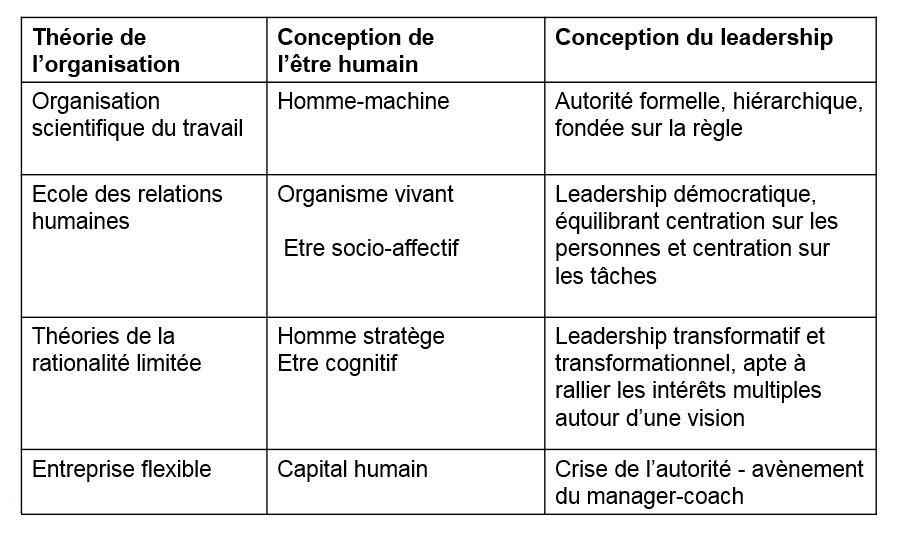
\includegraphics[scale=0.6]{conceptions_leaderships.png}
		\caption{Conceptions du leadership dans leur contexte historique.}
		\label{conceptions_leaderships}
		\end{center}
	\end{figure}
	
	
	\subsubsection{De l'autorité au leadership.}
	
	Le déclin du concept de l'autorité est lié aux nouveaux principes de la modernité démocratique:
	\begin{itemize}
	\item Égalité en droit et en dignité et libre expression de tous.
	\item Rationalisme contractuel dans les rapports humains.
	\item Raison scientifique et société de la connaissance.
	\item Dilution du pouvoir hiérarchique.
	\item Remise en cause du modèle bureaucratique.
	\item Crise du collectif et individualisme.
	\item Modification des relations familiales. \newline
	\end{itemize}
	
	Pour en savoir plus: conférence de Alain Eraly: L'avenir de l'autorité. \footnote{\url{http://enseignement.catholique.be/segec/index.php?id=1602}}
	
	\subsection{Définitions et approches}
	
	
	\subsection{Approche axée sur les traits}
	\subsection{Approche axée sur les comportements}
	\subsection{Approchée axée sur la situation}
	\subsection{Retour à des approches personnalisantes}
	

\section{La motivation au travail}
	\subsection{Définition}
		Être motivé, c'est
		\begin{itemize}
			\item Avoir un objectif ;
			\item Faire un effort pour l'atteindre ;
			\item Persévérer dans cet effort
		 \end{itemize}

		 Deux courants théoriques
		 \begin{itemize}
		 	\item théories des besoins, qu'est-ce qui motive ?
			\item théories des processus, comment est-on motivé ?
		 \end{itemize}

		 Qu'est-ce qui nous motive à travailler ?
		 \begin{itemize}
		 	\item Motivation extrinsèque = qui vient de l'extérieur (salaire, prime,...)
			\item Motivation intrinsèque = motivation en nous.
		 \end{itemize}
	\subsection{Histoire}
	\begin{enumerate}
		\item Conception instrumentale
		\item Conception humaniste
		\item Conception rationnelle
		\item Conception sociale
		\item Conception négociée
	\end{enumerate}

	\begin{description}
		\item[Conception instrumentale] : Mettre des moyens matériels pour motiver (\og{} Tout travail mérite salaire\fg{}, conception Tayloriste ou behavioriste)
		\item[Conception humaniste] : Ecole des relations humaines (\og{} Le travail c'est la santé\fg{}, les besoins fondamentaux sont reconnus)
		\item[Conception rationnelle] : L'humain est un acteur qui calcule ses intérêts (\og{} Le travail, un intérêt bien calculé\fg{} , approche socio-technique)
		\item[Conception sociale] : L'humain est motivé si la situation est juste d'un point de vue éthique (\og{} A travail égal, salaire égal\fg{}, justice)
		\item[Conception négociée] : Un contrat d'échange psychologique, fonction des attentes de chacun
	\end{description}
	\subsection{Conception instrumentale de la motivation}
	La conception instrumentale de la motivation prend place dans un contexte Tayloriste et behavioriste où le travail est extrêmement divisé (Organisation Scientifique du Travail). Pour rappel, le behaviorisme suppose que l'homme est naturellement paresseux, qu'il faut le mobiliser, lui donner des comportements adéquats (homme-machine). Cette conception s'appuie sur le principe de la \og{}loi de l'effet\fg{} (Stimulus $\Rightarrow$ Réponse) qui suppose que l'homme adopte automatiquement les comportements qui provoquent des effets qui lui sont favorables.

		\subsubsection{Principes du conditionnement}
			Le but est de conditionner le travailleur par des stimulus. On distingue 4 types de stimuli.
			
			\bigskip

			\begin{tabular}{|l|l|l|}
			\hline
			\textbf{Nom} & \textbf{Type de stimuli} & \textbf{Résultat} \\
			\hline
			Renforcement positif & Ajout d'un stimulus positif & Renforcement du comportement \\
			\hline
			Renforcement négatif & Supression d'un stimulus aversif & Renforcement du comportement \\
			\hline
			Extinction & Supression d'un stimulus positif & Diminution du comportement \\
			\hline
			Punition & Ajout d'un stimulus aversif & Diminution du comportement \\
			\hline
			\end{tabular}
			\bigskip

			On estime que le conditionnement est d'autant plus efficace si :
			
			\begin{itemize}
				\item Il est contingent (spontané) et répété
				\item Il est important (en quantité et en valeur)
				\item L'individu a été privé de ce conditionnement
				\item Il y a un renforcement fréquent et immédiat
			\end{itemize}
			
			Il est important de ne jamais laisser le travailleur libre (persistance et persévérance du conditionnement).

			% TODO : On pourrait ajout l'image page 13 de la synthèse LECGE1321.pdf


		\subsubsection{En pratique\ldots}
		Les pratiques à cette époque sont :
		
		\begin{itemize}
			\item Salaire à la pièce
			\item Prime de performance
			\item Intéressement au résultat
			\item Employé du mois
			\item Monitoring serré de la performance
		\end{itemize}

		Les ressources humaines ne travaillent qu'avec des motivations extrinsèques (salaire, récompense).

		\subsubsection{Effets de la conception instrumentale}
		\underline{Positif si} il y a de la conformité comportementale et la performance \og{} in role \fg{} (chacun son rôle).

		\underline{Nul ou négatif si} 
		
		\begin{itemize}
			\item l'identification à l'organisation et la performance extra-rôle ne sont pas promus à cette conception.
			\item s'il y a internalisation des valeurs de l'organisation et autonomie, initiave (effet extrinsèque nul
		\end{itemize}
		\begin{figure}[!ht]
			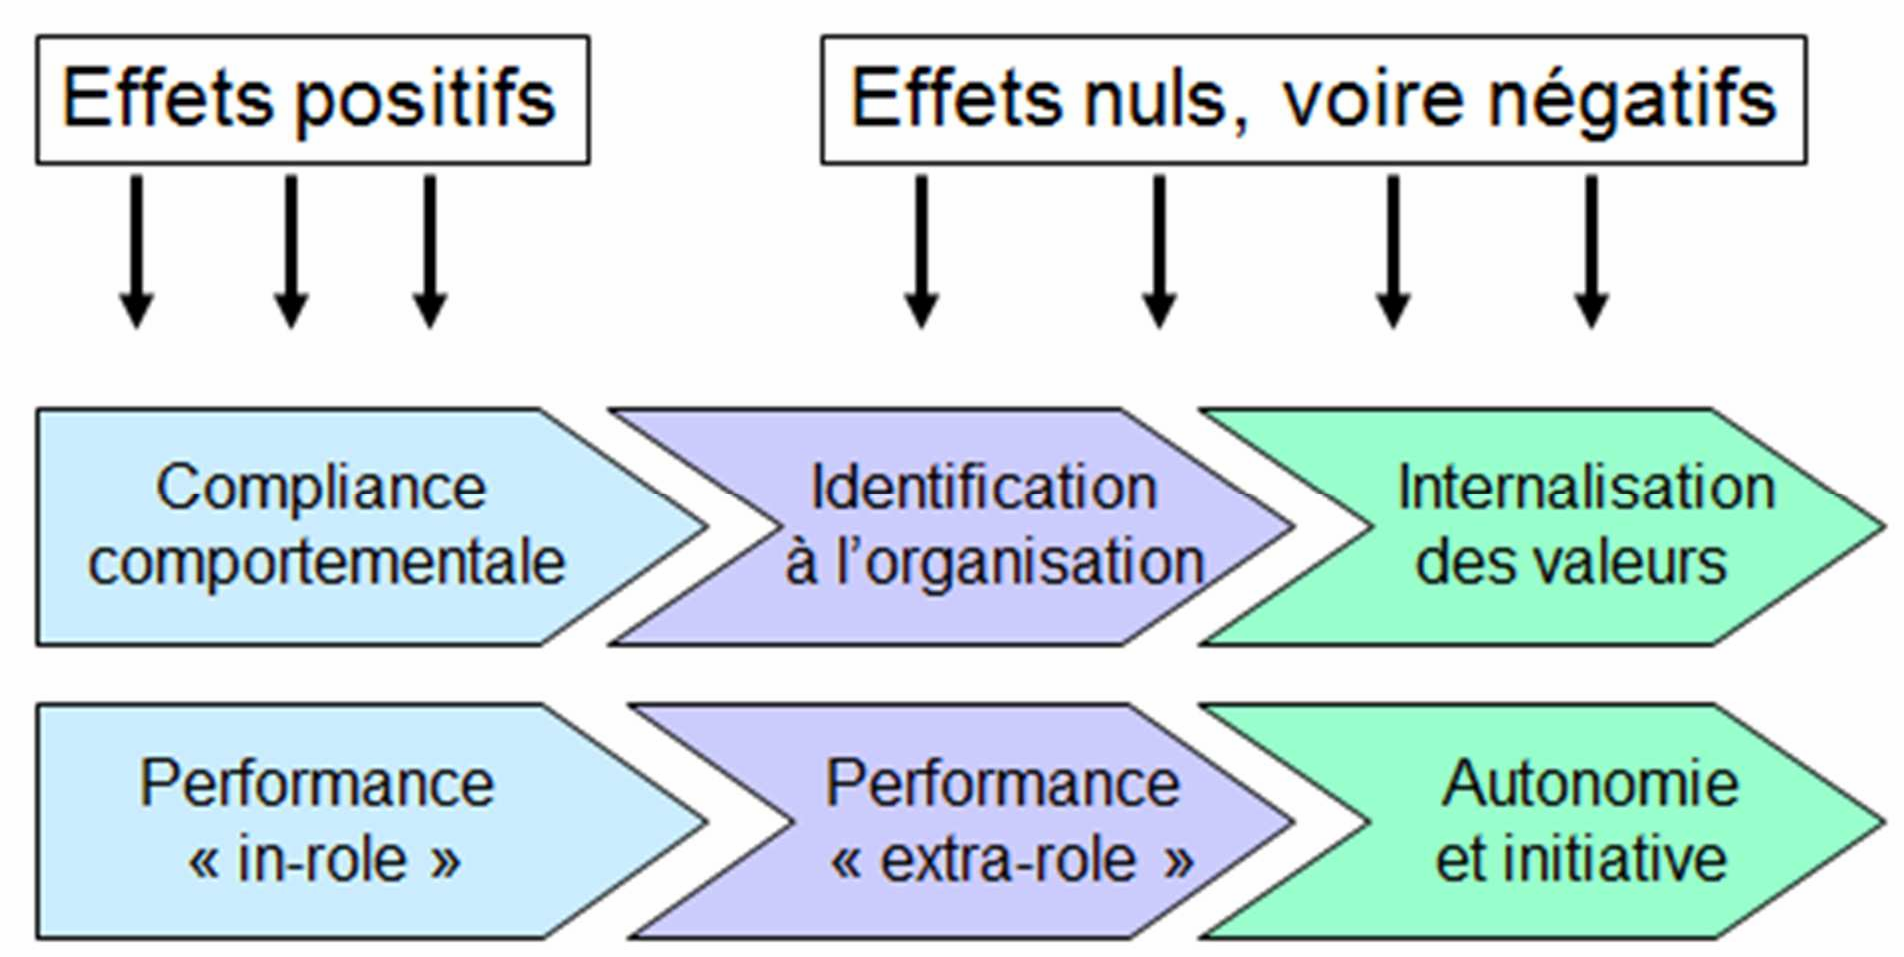
\includegraphics[width=\linewidth]{effets_de_la_conception_instrumentale.png}
			\caption{Effets de la conception instrumentale de la motivation}
		\end{figure}

	\subsection{Conception humaniste de la motivation}
	La conception humaniste de la motivation prend place dans un contexte de croissance économique dans lequel on tente de réhumaniser le travail. Le présupposé est que l'homme est un être vivant mu par des besoins.

	Cette conception s'appuie sur le principe de l'homéostasie. L'homéostasie s'appuie sur l'idée que l'homme a une capacité à garder un équilibre malgré les variations de son environnement. \newline 

	Besoin insatisfait $\Rightarrow$ Tension interne $\Rightarrow$ Motivation $\Rightarrow$ Assouvissement du besoin $\Rightarrow$ Réduction de la tension $\Rightarrow$ Satisfaction \newline

	Motivation $\neq$ Satisfaction $\Rightarrow$ Un besoin satisfait ne motive plus.

		\subsubsection{La pyramide de Maslow}
		Le but de ce modèle est d'établir une hiérarchisation des besoins de l'homme. Les besoins des hommes étant très changeant, ce modèle est faiblement robuste (il est peu durable dans le temps).

		\underline{Hypothèses :}
		\begin{enumerate}
			\item Un besoin satisfait ne peut plus motiver
			\item Les besoins supérieurs ne motivent que si les besoins inférieurs ont été comblés
			\item Universalité de la pyramide mais place spécifique de chacun dans la pyramide
		\end{enumerate}

		\bigskip

		\underline{Contenu :}

		\begin{enumerate}
			\item \textbf{Les besoins physiologiques} : préoccupation essentielle de survie qui priment sur les autres besoins (la nourriture, le repos, l'exercice et la sexualité)
				\subitem La société dans laquelle nous vivons oblige l'individu à travailler pour assouvir ces besoins
			\item \textbf{Les besoins de sécurité} : besoins liés à la protection immédiate et future de l'individu (sécurité de l'emploi, plans d'assurance, régime de retraite, protection contre l'injustice)
				\subitem Les besoins de sécurité des travailleurs sont en partie comblés avec un emploi permanent
			\item \textbf{Les besoins d'appartenance} : besoins d'une personne à faire partie d'associations ou de regroupements et de collaboration avec d'autres individus (amitié, affiliation, amour).
			\item \textbf{Les besoins d'estime} : estime de soi (confiance en soi, indépendance, épanouissement) et reconnaissance extérieure (considération, respect, promotion, valorisation)
			\item \textbf{Les besoins de réalisation} de soi (\og{}actualisation\fg{}) : besoin qu'éprouve une personne de réaliser ses aspirations, de se perfectionner et de créer au sens le plus large du terme.
		\end{enumerate}

		\begin{figure}[!ht]
			\begin{center}
			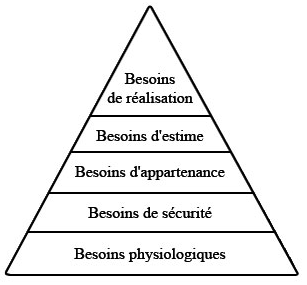
\includegraphics[width=0.5\linewidth]{pyramide_maslow.png}
			\caption{La pyramide de Maslow}
			\end{center}
		\end{figure}
		
		\underline{Limites :}
		\begin{itemize}
			\item La catégorisation des besoins ne peut être \og{} démontrée \fg{}. N'existe-t-il vraiment que cinq besoins ?
			\item Les liens entre les besoins ne sont pas prouvés. Il n'y a pas de lien négatif entre la satisfaction d'un besoin et la force de la motivation
			\item Cette représentation ne dit pas comment expliquer la démovitation ?
			\item Dans cette vision hiérarchique, quel est l'impact des contextes culturels et organisationnels ?
		\end{itemize}

		\subsubsection{Le modèle bi-factoriel de Herzberg}
		Méthodologie de l'étude (1959) \og{}The Motivation to Work\fg{}
		\begin{itemize}
			\item 200 employés interviewés chez AT\&T (ingénieurs et comptables)
			\item \underline{But :} Vérifier l'hypothèse selon laquelle certains facteurs étaient satisfaisant alors que d'autres provoquaient strictement l'insatisfaction.
			\item Techniques des incidents critiques (Flanagan, 1954) : Un incident critique se définit comme un évènement ayant eu une causalité importante sur le résultat final d'une activité. Ces incidents critiques ne peuvent donc être reconnus qu'a posteriori. Le but est d'expliquer la conduite de la personne en activité et les difficultés qu'elle rencontre.
		\end{itemize}

		\begin{figure}[!ht]
			\begin{center}
			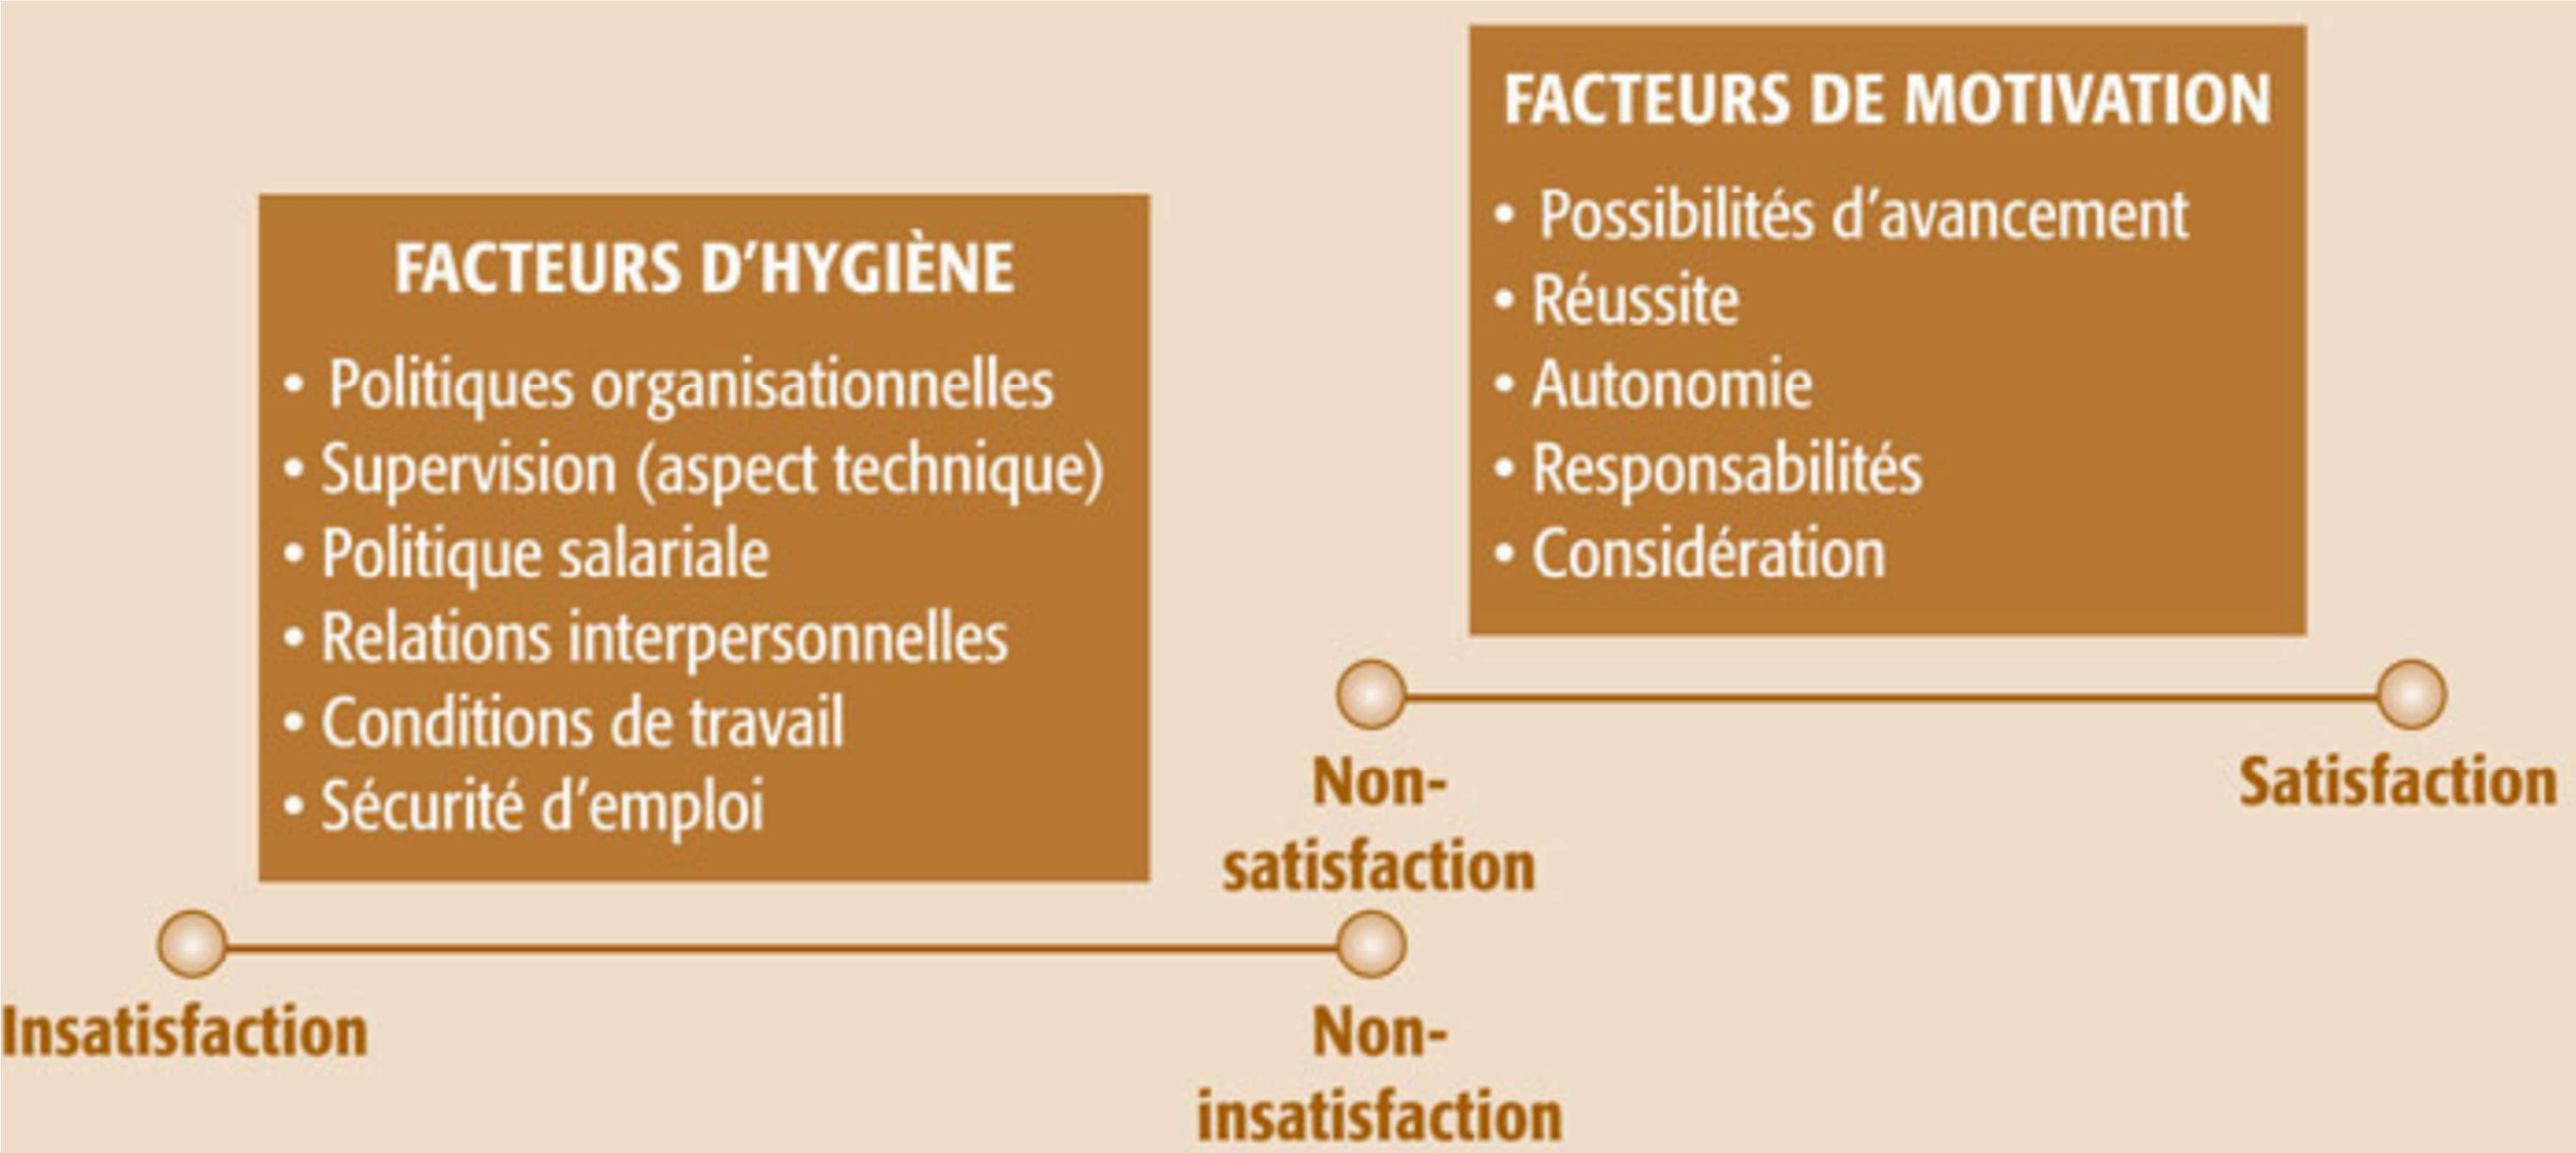
\includegraphics[width=\linewidth]{facteurs_herzberg.png}
			\caption{Modèle bi-factoriel de Herzberg}
			\end{center}
		\end{figure}
		
		Il y a deux sortes de facteurs :
		\begin{enumerate}
			\item \textbf{Ceux qui permettent de réduire l'insatisfaction} pour arriver au point neutre.
				\subitem Facteurs plutôt extrinsèques (politique et gestion RH, sécurité d'emploi,...)
			\item \textbf{Ceux qui permettent de réellement de motiver} : lié au contenu de la tâche.
				\subitem Facteurs plutôt intrinsèques
		\end{enumerate}

		\begin{figure}[!ht]
		\begin{center}
			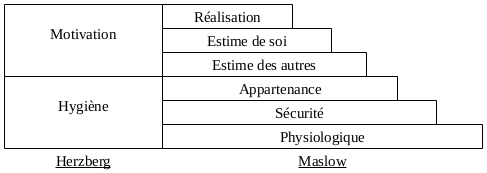
\includegraphics[width=0.6\linewidth]{herzberg_vs_maslow.png}
			\caption{Comparaison des modèles Herzberg et Maslow}
		\end{center}
		\end{figure}

		\subsubsection{La théorie de McClelland}
		\subsubsection{La théorie ESC d’Alderfer (1969)}
		\subsubsection{En pratique… L’enrichissement du travail}
		\subsubsection{Effets de la conception humaniste}
	\subsection{Conception rationnelle de la motivation}
		\subsubsection{Les théories de processus}
		\subsubsection{Le modèle de room : la théorie des attentes}
		\subsubsection{En pratique}
		\subsubsection{Théorie de l’effet de but (Locke, 1968)}
		\subsubsection{Management by objectives (P. Drucker, 1954)}
		\subsubsection{Effet de la conception rationnelle}
	\subsection{Conception sociale de la motivation}
		\subsubsection{La théorie de l’équipe d’Adams}
		\subsubsection{En pratique}
		\subsubsection{Effets de la conception sociale}
		\subsubsection{Justice organisationnelle (Greenberg 1987)}
	\subsection{Et aujourd’hui…}
		Comment peut-on encore encourager la motivation et l’implication du personnel ?
		\subsubsection{Dans quel paysage travaillons-nous ?}
		\subsubsection{Formes traditionnelles du contrat psychologique}
		\subsubsection{Effets du contrat psychologique}
		\subsubsection{Formation et rupture du contrat psychologique}
		\subsubsection{Effets de la conception négociée}
		\subsubsection{En pratique…}
		\subsubsection{Que retenir ?}

\section{Conclusion}

\bibliographystyle{plain}
\bibliography{biblio}


\end{document}
